\documentclass[11pt,letterpaper]{article}
\usepackage{amsmath,amssymb,amsthm}
\usepackage{mathtools}
\usepackage{geometry}
\usepackage{graphicx}
\usepackage{booktabs}
\usepackage{hyperref}
\usepackage{bm}
\usepackage{xcolor}
\usepackage{cleveref}
\usepackage{enumitem}
\usepackage{float}
\usepackage{longtable}
\usepackage{subcaption}

\graphicspath{{figures/sim_excitation/}}

\geometry{margin=1.1in}

\hypersetup{
  colorlinks=true,
  linkcolor=blue!70!black,
  citecolor=green!50!black,
  urlcolor=blue,
  hypertexnames=false
}

\newcommand{\diff}{\mathrm{d}}
\newcommand{\deriv}[2]{\frac{\diff #1}{\diff #2}}
\newcommand{\pderiv}[2]{\frac{\partial #1}{\partial #2}}
% \ddot is already defined by LaTeX — use standard \ddot{x} directly
\newcommand{\eq}[1]{\textcolor{blue!70!black}{#1}}

\title{\textbf{Mathematical Derivation of Bistable Mechanisms\\for Vibration-Triggered Hook Deployment}\\[0.5em]
\large Rolly Robot --- Hook Bistable Actuator Simulations}
\author{Technical note for the Rolly hook-deployment simulations}
\date{2026}

\begin{document}
\maketitle
\tableofcontents
\newpage

%%─────────────────────────────────────────────────────────────────────────────
\section{Introduction}
\label{sec:intro}
%%─────────────────────────────────────────────────────────────────────────────

A \emph{bistable} mechanical system has two stable equilibrium positions
separated by an energy barrier. If it is not disturbed, it stays in whichever
well it already occupies. Moving from one well to the other requires enough
input energy to cross the intervening saddle; the rapid transition is the
\emph{snap-through} event~\cite{qiu2004,liu2023}.

For the Rolly hook, the first well holds the hook retracted. A RobStride RS05
quasi-direct-drive motor drives the surrounding structure with a sinusoidal
force or displacement. Near resonance, the hook motion grows until the relative
coordinate crosses the saddle. After snap-through the second well holds the hook
deployed without continuous motor power. The model here is therefore concerned
with three quantities: the barrier height, the natural frequency about the
retracted state, and the actuator amplitude needed to reach the saddle.

The physical model derived and simulated here is \textbf{Simulation 2 (Physical)}: a
compliant curved-beam bistable mechanism following the geometry of Qiu et al.~\cite{qiu2004}
and the 3D-printed Design~9 of Zolfagharian et al.~\cite{zolfagharian2025}, with a companion
two-degree-of-freedom tuned mass damper (TMD) model~\cite{denhartog1956}.

\subsection{Variable Map}
\label{ssec:variables_plain}

The MATLAB scripts use compact variable names. The table below gives the
mechanical meaning of the variables that drive the model.

\begin{table}[H]
\centering
\caption{Plain-language map between MATLAB names and model variables.}
\renewcommand{\arraystretch}{1.25}
\begin{tabular}{p{3.1cm} p{3.1cm} p{7.2cm}}
\toprule
\textbf{MATLAB name} & \textbf{Symbol} & \textbf{Meaning} \\
\midrule
\texttt{h\_apex} & $h$ & Beam arch height at mid-span before snap. This sets the arch shape and the $Q$ ratio. \\
\texttt{t\_beam} & $t$ & Beam thickness. A thicker beam lowers $Q=h/t$ but increases stiffness. \\
\texttt{l\_span} & $l$ & Hinge-to-hinge beam span. \\
\texttt{Q\_beam}, \texttt{Q} & $Q=h/t$ & Bistability ratio. The scripts now require $Q\geq2.35$. \\
\texttt{n\_cells} & $N$ & Number of parallel bistable beams in the pack. Parallel beams share displacement and add force/stiffness. \\
\texttt{d\_stroke\_1cell} & $d_{f,1}$ & Single-beam travel from retracted State~1 to deployed State~2. \\
\texttt{d\_stroke} & $d_f$ & Mechanism travel used by the ODE. In the parallel model this equals \texttt{d\_stroke\_1cell}. \\
\texttt{d\_saddle} & $d_s$ & Unstable saddle displacement. Crossing this displacement triggers snap-through. \\
\texttt{F\_push\_1cell} & $F_{\mathrm{push},1}$ & Peak force for one beam. The beam-pack force is $N F_{\mathrm{push},1}$. \\
\texttt{A\_coeff} & $A$ & Cubic force coefficient in $F_{\mathrm{restore}}=-A d(d-d_s)(d-d_f)$. \\
\texttt{k\_eff\_s1} & $k_{\mathrm{eff},1}$ & Linearized stiffness near the retracted well. This sets $f_{n,1}$. \\
\texttt{m\_hook} & $m_h$ & Hook/reference mass attached to the bistable mechanism. \\
\texttt{M\_plate} & $M_P$ & Moving plate/structure mass used in the base-excitation model. \\
\texttt{xP} & $x_P$ & Absolute plate displacement. \\
\texttt{xr}, \texttt{x\_rel} & $x_{\mathrm{rel}}$ & Hook displacement relative to the plate. Snap occurs when this crosses $d_s$. \\
\texttt{A\_min\_c2} & $A_{\min}$ & Minimum prescribed plate amplitude for Config~2 snap in the linear estimate. \\
\bottomrule
\end{tabular}
\end{table}

%%─────────────────────────────────────────────────────────────────────────────
\section{Compliant Curved-Beam Bistable Mechanism}
\label{sec:sim2}
%%─────────────────────────────────────────────────────────────────────────────

\subsection{Beam Geometry --- Qiu Cosine Profile}
\label{ssec:geometry}

Qiu et al.~\cite{qiu2004} proposed the initial (stress-free) shape of the
curved beam as the first buckling mode of a fixed-end Euler beam, a
cosine profile:
\begin{equation}
  y_0(\xi) = \frac{h}{2}\left[1 - \cos\!\left(\frac{2\pi\xi}{l}\right)\right],
  \quad 0 \leq \xi \leq l
  \label{eq:beamprofile}
\end{equation}
where $h$ is the apex height [m] and $l$ is the horizontal span [m]. The beam
thickness is $t$ [m], and the material elastic modulus is $E$ [Pa].

Key geometric parameters:
\begin{align}
  Q &= \frac{h}{t} \quad\text{(apex-height-to-thickness ratio)} \label{eq:Qdef}\\
  I &= \frac{t^3}{12} \quad\text{(second moment of area per unit width)} \label{eq:Idef}
\end{align}

\subsection{Bistability Condition}
\label{ssec:bistability_condition}

For a curved beam to exhibit bistability, two design conditions matter most
\cite{qiu2004,zolfagharian2025}:

\begin{enumerate}
  \item \textbf{Q-ratio condition}: The apex height must substantially exceed
    the beam thickness:
    \begin{equation}
      Q = \frac{h}{t} \gtrsim 2.35
      \label{eq:Qcond}
    \end{equation}
    Qiu et al.\ report that a second-mode-constrained curved beam becomes
    bistable once this geometric ratio is large enough; their analysis and
    force-displacement plots put the threshold at about $Q=2.35$
    \cite{qiu2004}. The MATLAB model now enforces $Q\geq2.35$ directly.

  \item \textbf{Mode-2 suppression}: For a single beam, buckling mode~2 is
    asymmetric and prevents robust bistability. In the Zolfagharian Design~9, a
    \emph{double-curved beam} connected by a central membrane at mid-span
    suppresses mode~2, so the snap-through path follows the symmetric
    constrained-beam behavior described by Qiu et al.~\cite{qiu2004}.
\end{enumerate}

\subsection{Force-Displacement Relationship}
\label{ssec:FD}

\subsubsection{Strain Energy Formulation}

Using the Euler--Bernoulli beam assumptions, let the initial shape be
$y_0(\xi)$ and the transverse displacement from that shape be $w(\xi)$, so
$y(\xi) = y_0(\xi) - w(\xi)$ where $w$ is the transverse displacement
relative to the initial shape. The bending strain energy is then
\cite{qiu2004}:
\begin{equation}
  U_b = \frac{EI}{2}\int_0^l \left(\frac{\diff^2 w}{\diff\xi^2}\right)^2\diff\xi
  \label{eq:Ub}
\end{equation}
The axial compressive strain energy (due to shortening of the beam's projected
length) is:
\begin{equation}
  U_a = \frac{EA}{2l}\left(\int_0^l \frac{\diff y_0}{\diff\xi}
        \frac{\diff w}{\diff\xi}\,\diff\xi\right)^2
  \label{eq:Ua}
\end{equation}
where $A = t\cdot b$ is the cross-sectional area (for width $b$).

The force-displacement relationship follows from virtual work:
$F = \partial(U_b + U_a)/\partial d$, where $d$ is the mid-point displacement
(snapping direction).

\subsubsection{Normalized Force-Displacement}

Qiu et al.~\cite{qiu2004} show that the force-displacement curve depends
only on $Q$ and the normalized displacement $\bar{d} = d/h$. For the
double-beam (mode-2 suppressed) configuration, the curve has the
characteristic S-shape:
\begin{itemize}[nosep]
  \item \textbf{State 1} ($\bar{d} = 0$): zero force (equilibrium).
  \item \textbf{Peak push force} $F_{\mathrm{push}}$ at $\bar{d} \approx 0.27$:
    maximum force required to initiate snap-through.
  \item \textbf{Saddle} ($\bar{d} = \bar{d}_s$): force returns to zero
    (unstable equilibrium).
  \item \textbf{Valley force} $F_{\mathrm{pop}} < 0$ at $\bar{d} \approx 0.82$:
    mechanism pulls itself toward State~2.
  \item \textbf{State 2} ($\bar{d} = 1$): zero force (second equilibrium).
\end{itemize}

\subsubsection{Cubic Polynomial Fit}
\label{sssec:cubic}

The simulation uses a cubic fit for the applied force in the compression-test
convention. This is not a replacement for Qiu's modal solution or
Zolfagharian's FEA; it is a compact surrogate with the correct equilibrium
points and peak force:
\begin{equation}
  F_{\mathrm{ext}}(d) = A\,d\,(d - d_s)\,(d - d_f)
  \label{eq:Fext_cubic}
\end{equation}
The coefficient $A$ is calibrated so the force at the chosen peak location
matches the Design~9 force level from Zolfagharian et al.~\cite{zolfagharian2025}:
\begin{equation}
  A = \frac{F_{\mathrm{push}}}{d_{\mathrm{push}}\,(d_{\mathrm{push}} - d_s)\,(d_{\mathrm{push}} - d_f)}
  \label{eq:Acoeff}
\end{equation}
where $d_{\mathrm{push}} \approx 0.27\,d_f$ is the location of the force peak.

The \emph{internal restoring force} on an attached mass (Newton's third law)
is:
\begin{equation}
  F_{\mathrm{restore}}(d) = -F_{\mathrm{ext}}(d) = -A\,d\,(d - d_s)\,(d - d_f)
  \label{eq:Frestore2}
\end{equation}

\subsection{Potential Energy (Curved-Beam Model)}
\label{ssec:potential2}

Integrating the restoring force analytically:
\begin{align}
  V(d) &= -\int_0^d F_{\mathrm{restore}}(\xi)\,\diff\xi
         = A\int_0^d \xi\,(\xi-d_s)\,(\xi-d_f)\,\diff\xi \notag\\
       &= A\int_0^d \bigl[\xi^3 - (d_s+d_f)\xi^2 + d_s d_f\,\xi\bigr]\diff\xi \notag\\
       &= A\left[\frac{d^4}{4} - \frac{(d_s+d_f)}{3}d^3 + \frac{d_s d_f}{2}d^2\right]
  \label{eq:V2}
\end{align}
The energy barrier from State~1 to the saddle is:
\begin{equation}
  \Delta E_1 = V(d_s) - V(0)
  = A\left[\frac{d_s^4}{4} - \frac{(d_s+d_f)}{3}d_s^3 + \frac{d_s d_f}{2}d_s^2\right]
  \label{eq:barrier2}
\end{equation}

\subsection{Natural Frequencies at Each Stable State}
\label{ssec:natfreq2}

Linearizing $F_{\mathrm{restore}}(d)$ about each equilibrium:

\textbf{State 1} ($d = 0$):
\begin{equation}
  k_{\mathrm{eff,1}} = \left.-\frac{\diff F_{\mathrm{restore}}}{\diff d}\right|_{d=0}
  = A\,d_s\,d_f
  \label{eq:keff1}
\end{equation}
\begin{equation}
  \omega_{n,1} = \sqrt{\frac{k_{\mathrm{eff,1}}}{m}}, \qquad
  f_{n,1} = \frac{1}{2\pi}\sqrt{\frac{A\,d_s\,d_f}{m}}
  \label{eq:fn1}
\end{equation}

\textbf{State 2} ($d = d_f$):
\begin{equation}
  k_{\mathrm{eff,2}} = \left.-\frac{\diff F_{\mathrm{restore}}}{\diff d}\right|_{d=d_f}
  = A\,d_f\,(d_f - d_s)
  \label{eq:keff2}
\end{equation}
\begin{equation}
  \omega_{n,2} = \sqrt{\frac{k_{\mathrm{eff,2}}}{m}}, \qquad
  f_{n,2} = \frac{1}{2\pi}\sqrt{\frac{A\,d_f\,(d_f - d_s)}{m}}
  \label{eq:fn2}
\end{equation}

Since $d_s < d_f$ by definition, and typically $d_s \approx 0.55\,d_f$:
$k_{\mathrm{eff,2}} = A\,d_f(d_f-d_s) \approx 0.45\,A\,d_f^2$, while
$k_{\mathrm{eff,1}} = A\,d_s\,d_f \approx 0.55\,A\,d_f^2$, so
$k_{\mathrm{eff,2}} < k_{\mathrm{eff,1}}$ and thus $f_{n,2} < f_{n,1}$.

\subsection{Parallel Beam-Pack Mechanics}
\label{ssec:stacked}

The robot layout is treated as a parallel pack of identical curved beams. The
beams share the same hook displacement, so adding beams does \emph{not} add
stroke. Instead, the force and stiffness add:
\begin{align}
  d_{f,N} &= d_{f,1} \quad\text{(same stroke)} \label{eq:stackstroke}\\
  d_{s,N} &= d_{s,1} \quad\text{(same saddle position)} \label{eq:stacksaddle}\\
  F_{\mathrm{push},N} &= N\,F_{\mathrm{push},1}
\end{align}

The coefficient $A$ for the beam pack therefore scales linearly:
\begin{equation}
  A_N = N\,A_1
  \label{eq:AN}
\end{equation}
because the displacement terms in the cubic polynomial are unchanged while the
force is multiplied by $N$. The effective stiffnesses scale the same way:
\begin{equation}
  k_{\mathrm{eff,1},N} = A_N\,d_s\,d_f = N\,k_{\mathrm{eff,1},1}
  \label{eq:keffN}
\end{equation}
Thus adding parallel beams raises the natural frequency:
\begin{equation}
  f_{n,1,N} = \sqrt{N}\,f_{n,1,1}
  \label{eq:fnN}
\end{equation}
This correction keeps the saddle displacement on the order of a single beam's
travel, not five times that travel.

\subsection{1-DOF Hook Snap-Through Model}
\label{ssec:1dof}

The hook mass $m$ is connected to the fixed robot body through the bistable
mechanism. External vibration $F_{\mathrm{exc}}(t)$ is transmitted through
the robot structure. The equation of motion is:
\begin{equation}
  m\ddot{d} + c\,\dot{d} + F_{\mathrm{restore}}(d) = F_{\mathrm{exc}}(t)
  \label{eq:1dof2}
\end{equation}
where $c = 2\zeta m\omega_{n,1}$. The excitation is a linear chirp
(frequency-modulated sinusoid):
\begin{equation}
  F_{\mathrm{exc}}(t) = F_0\sin\!\left[2\pi\!\left(f_{\mathrm{lo}}\,t
    + \frac{f_{\mathrm{hi}} - f_{\mathrm{lo}}}{2t_f}t^2\right)\right]
  \label{eq:chirp}
\end{equation}
where $f_{\mathrm{lo}}$, $f_{\mathrm{hi}}$ are the chirp bounds [Hz] and
$t_f$ is the simulation duration [s]. As the instantaneous frequency passes
through $f_{n,1}$, resonance amplifies the displacement until snap-through.

\subsection{2-DOF Tuned Mass Damper Model}
\label{ssec:2dof}

Following Zolfagharian et al.~\cite{zolfagharian2025} (their Figure~4), the
main structure mass $m_1$ is supported by spring $k_{\mathrm{main}}$ and
driven harmonically. The TMD mass $m_2$ is attached to the same flexible ruler
at distance $L_2$ from the fixed end, where the bistable mechanism
repositions it.

The coupled equations of motion are:
\begin{align}
  m_1\ddot{x}_1 + c_{\mathrm{main}}\dot{x}_1 + k_{\mathrm{main}}x_1
    + k_b(x_1 - x_2) + c_b(\dot{x}_1 - \dot{x}_2) &= F_0\sin(\omega t)
  \label{eq:2dof1}\\
  m_2\ddot{x}_2 - k_b(x_1 - x_2) - c_b(\dot{x}_1 - \dot{x}_2) &= 0
  \label{eq:2dof2}
\end{align}
where $k_b$ and $c_b$ are the stiffness and damping of the bistable TMD
connection, linearized at the current stable state.

\subsubsection{Stiffness of the Flexible Ruler}

The effective spring stiffness of a flexible cantilever beam (ruler) at
distance $L$ from the fixed support is~\cite{zolfagharian2025}:
\begin{equation}
  k = \frac{3EI_r}{L^3}
  \label{eq:rulerspring}
\end{equation}
where $E_r$ is the ruler's elastic modulus, $I_r$ is its second moment of area.
When the bistable mechanism shifts the TMD mass from $L_1$ to $L_2 = L_1 + d_f$:
\begin{equation}
  k_{\mathrm{TMD,2}} = \frac{3E_r I_r}{L_2^3}
                     = \frac{3E_r I_r}{(L_1 + d_f)^3}
                     < k_{\mathrm{TMD,1}}
  \label{eq:kTMDshift}
\end{equation}
This reduction in TMD stiffness shifts the TMD natural frequency downward,
changing the frequency at which it suppresses main-mass vibration.

\subsubsection{Steady-State Frequency Response}

In the frequency domain, the steady-state response of $x_1$ to
$F_0 e^{i\omega t}$ is $X_1 e^{i\omega t}$. The impedance formulation gives:
\begin{equation}
  \begin{bmatrix} Z_{11} & Z_{12} \\ Z_{21} & Z_{22} \end{bmatrix}
  \begin{Bmatrix} X_1 \\ X_2 \end{Bmatrix} =
  \begin{Bmatrix} F_0 \\ 0 \end{Bmatrix}
  \label{eq:impedance}
\end{equation}
where
\begin{align}
  Z_{11} &= (k_{\mathrm{main}} + k_b - m_1\omega^2) + i\omega(c_{\mathrm{main}} + c_b) \\
  Z_{12} &= Z_{21} = -(k_b + i\omega c_b) \\
  Z_{22} &= (k_b - m_2\omega^2) + i\omega c_b
\end{align}
Solving by Cramer's rule:
\begin{equation}
  X_1 = \frac{F_0\,Z_{22}}{Z_{11}Z_{22} - Z_{12}^2}
  \label{eq:X1}
\end{equation}
The amplitude $|X_1(\omega)|$ vs.\ $\omega/(2\pi)$ [Hz] is plotted for three
configurations: no TMD, TMD in State~1, TMD in State~2.

%%─────────────────────────────────────────────────────────────────────────────
\section{Base Excitation via Motor Torque Oscillation Through Shared Structure}
\label{sec:baseexcit}
%%─────────────────────────────────────────────────────────────────────────────

\subsection{Physical Setup}
\label{ssec:setup_base}

\subsubsection{Mechanism component chain}

The Zolfagharian Design~9 bistable mechanism consists of the following rigid
bodies connected in series:

\begin{enumerate}[nosep]
  \item \textbf{Robot chassis / ground} --- the fixed reference frame.
  \item \textbf{Spring isolators} ($k_s$, $c_s$) --- soft mounting elements
    (rubber mounts, vibration isolators) between the chassis and the plate
    assembly.
  \item \textbf{Rigid plate assembly} ($M_P$) --- one rigid body comprising the
    plate, the motor housing, and the \emph{external blocks}.  The external
    blocks are the side walls to which the bistable beam ends are pinned.
  \item \textbf{Bistable curved beams} --- the compliant Qiu cosine-profile beams
    spanning between the external blocks.  These provide the nonlinear
    restoring force $F_{\mathrm{restore}}(x_{\mathrm{rel}})$ and potential
    energy $V(x_{\mathrm{rel}})$.
  \item \textbf{Hook} ($m_h$, also called the \emph{reference mass}) --- the
    deployable element attached at the beam apex.  In State~1 the beam is
    arched and the hook is retracted; in State~2 the beam has snapped through
    and the hook is deployed.
\end{enumerate}

\noindent The hook is connected to the plate assembly \emph{only} through the
bistable beams --- there is no rigid link.  When the plate assembly vibrates,
the hook cannot follow instantaneously; the resulting \textbf{relative
displacement} $x_{\mathrm{rel}}$ between the beam apex (hook) and the beam ends
(external blocks on plate) is the quantity that drives snap-through.

\begin{figure}[H]
\centering
\begin{verbatim}
  ROBOT CHASSIS
        |
        |  k_s, c_s   <- spring isolators / rubber feet
        |
  RIGID ASSEMBLY  (M_P = motor + plate + external blocks)
        |                  external blocks = beam end pinned supports
        |
      BEAM      BEAM    <- bistable curved beams (Qiu cosine profile)
        |          |
        +----+-----+
             |
           HOOK  (m_h = reference mass at beam apex)
\end{verbatim}
\caption{Physical component chain for the Zolfagharian bistable deployment
         mechanism.}
\label{fig:chain}
\end{figure}

\subsubsection{Two excitation configurations}

\paragraph{Configuration~1 --- Motor on plate assembly.}
The motor housing is bolted directly to the plate (part of $M_P$).  The
motor shaft drives an eccentric mass or proof mass whose reaction force
enters the plate through the bearing.  The plate assembly vibrates; the hook
responds via base excitation through the beams.
$$\text{Motor} \;\to\; \text{Plate} + \text{External blocks} \;\to\;
  \text{Beams} \;\to\; \text{Hook}$$

\paragraph{Configuration~2 --- Motor off plate, drives via bearing.}
The motor housing is \emph{not} part of the plate assembly.  The motor output
shaft drives the plate+external-blocks assembly directly through a bearing
coupling (lever arm, crank, or shaft).  In this configuration the motor can
\emph{prescribe} the plate displacement:
$$x_P(t) = A\,\sin(\omega_{n,1}\,t)$$
The hook responds to this base excitation through the beams.  The motor
housing mass is excluded from $M_P$.
$$\text{Motor} \;\to\; \text{Bearing} \;\to\;
  \text{Plate} + \text{External blocks} \;\to\; \text{Beams} \;\to\; \text{Hook}$$

Configuration~2 avoids the tuned-mass-damper anti-resonance problem because the
motor enforces the plate amplitude regardless of the hook's dynamics.

\subsubsection{Coordinates}

Two coordinate systems are used throughout:
\begin{itemize}[nosep]
  \item $x_P(t)$: absolute displacement of the rigid plate assembly [m]
    (positive in the snap direction, i.e.\ from State~1 toward State~2)
  \item $x_H(t)$: absolute hook displacement [m]
  \item $x_{\mathrm{rel}}(t) \equiv x_H(t) - x_P(t)$: hook displacement
    \emph{relative to the plate assembly} [m] --- this is the quantity that
    enters the bistable restoring force and potential energy
\end{itemize}

Snap-through occurs when $x_{\mathrm{rel}}$ crosses the saddle point
$d_s$ with positive velocity.

%%─────────────────────────────────────────────────────────────────────────────
\subsection{Motor Torque Excitation Force}
\label{ssec:torqueexcit}

In torque/current control mode the RS05 applies a sinusoidal output torque
$\tau_{\mathrm{out}}(t)$.  Through a coupling of moment arm $r_{\mathrm{arm}}$
[m] this becomes a linear force on the plate:
\begin{equation}
  F_{\mathrm{motor}}(t) = \frac{\tau_{\mathrm{out}}}{r_{\mathrm{arm}}}\,\sin(\omega_d t)
  \equiv F_0\,\sin(\omega_d t)
  \label{eq:Ftorque}
\end{equation}
where $\tau_{\mathrm{out}}$ is the \textbf{measured output torque} read from the
motor's torque--speed (T-N) curve at the instantaneous operating condition, and
$\omega_d$ is the drive frequency set by the controller command.  The amplitude
$F_0$ is therefore \emph{independent of frequency} --- a key difference from a
rotating-unbalance source whose amplitude grew as $\omega^2$.

For a linear chirp sweep from $f_{\mathrm{lo}}$ to $f_{\mathrm{hi}}$ over total
time $t_f$, the instantaneous frequency and accumulated phase are:
\begin{align}
  f_{\mathrm{inst}}(t) &= f_{\mathrm{lo}} + \frac{f_{\mathrm{hi}} - f_{\mathrm{lo}}}{t_f}\,t
  \label{eq:finst}\\
  \varphi(t) &= 2\pi\!\left[f_{\mathrm{lo}}\,t
    + \frac{f_{\mathrm{hi}} - f_{\mathrm{lo}}}{2t_f}\,t^2\right]
  \label{eq:phi}
\end{align}
The torque-driven force during a chirp is:
\begin{equation}
  F_{\mathrm{motor}}(t) = F_0\,\sin(\varphi(t))
  \label{eq:FtorqueChirp}
\end{equation}
The amplitude envelope $F_0$ is constant throughout the sweep, so the force
delivered at $f_{n,1}$ equals the force at any other frequency in the band ---
the mechanism receives full excitation amplitude at every point in the chirp.

%%─────────────────────────────────────────────────────────────────────────────
\subsection{Gearbox Effects on Vibration Transmission}
\label{ssec:gearbox}

Any gearbox in the drivetrain between the motor rotor and the bistable plate
acts as a mechanical filter.  The gear ratio $n_g$ amplifies the rotor's
reflected inertia and creates a low-pass cut-off frequency above which
vibrations are attenuated before reaching the plate.  Two architectures
relevant to bistable excitation are treated below.

%%─────────────────────────────────────────────────────────────────────────────
\subsubsection{Planetary Gearboxes}
\label{sssec:planetary}

A planetary gearbox achieves its ratio $n_g$ through a sun--planet--ring
arrangement.  Typical ratios range from 3:1 to about 20:1 per stage; multi-stage
units reach 100:1.  QDD motors use a single low-ratio planetary stage
($n_g \lesssim 10$) specifically to preserve backdrivability and broadband force
transmission.

\textbf{Reflected rotor inertia.}  At the output shaft, the effective inertia is:
\begin{equation}
  J_{\mathrm{eff}} = J_{\mathrm{rotor}}\,n_g^2 + J_{\mathrm{gears}} + J_{\mathrm{output}}
  \label{eq:Jeff}
\end{equation}
The $n_g^2$ factor dominates: even a modest 5:1 ratio makes the rotor inertia
appear $25\times$ larger at the output.  Combined with the finite gear-mesh
stiffness $k_{\mathrm{gear}}$, this creates a mechanical low-pass cut-off
frequency:
\begin{equation}
  f_{\mathrm{cut}} \approx \frac{1}{2\pi}\sqrt{\frac{k_{\mathrm{gear}}}{J_{\mathrm{eff}}}}
  \label{eq:fcut}
\end{equation}
Vibrations at frequencies above $f_{\mathrm{cut}}$ are attenuated before
reaching the plate; those well below $f_{\mathrm{cut}}$ pass through with
little attenuation.  A low gear ratio keeps $f_{\mathrm{cut}}$ high, so the
motor remains substantially backdrivable and transmits a broad vibration
band --- a favorable property for this application.

\textbf{Design rule:} verify that $f_{n,1} < f_{\mathrm{cut}}$ so that the
bistable resonance lies in the pass-band of the actuator's mechanical filter.
This check should use the actual mounted motor and linkage geometry, not the
bare motor datasheet value.

\textbf{Gear-mesh frequency.}  The planet-gear tooth contacts produce a
secondary vibration at:
\begin{equation}
  f_{\mathrm{mesh}} = n_g\,f_{\mathrm{rotor}}\,N_{\mathrm{teeth}}
  \label{eq:fmesh}
\end{equation}
where $N_{\mathrm{teeth}}$ is the planet tooth count.  If $f_{\mathrm{mesh}}$
happens to coincide with $f_{n,1}$, this harmonic can contribute beneficially to
snap-through excitation without any additional control effort.  A low single-stage
ratio keeps $f_{\mathrm{mesh}}$ well above the bistable resonance band, avoiding
unintended parametric excitation.

%%─────────────────────────────────────────────────────────────────────────────
\subsubsection{High-Ratio Straight-Tooth Gearboxes}
\label{sssec:highratiospur}

Multi-stage spur or helical gearboxes achieve ratios of $n_g = 20$:1 to
$n_g > 100$:1 by cascading two or more stages of spur (straight-tooth) or
helical gears.  They are inexpensive and compact relative to harmonic or
cycloidal alternatives at the same ratio, but carry two significant penalties
for bistable vibration excitation.

\textbf{Reflected inertia penalty.}  Because $n_g$ is large, the $n_g^2$ term
in \cref{eq:Jeff} dominates overwhelmingly.  The cut-off frequency $f_{\mathrm{cut}}$
drops accordingly:
\begin{equation}
  f_{\mathrm{cut}} \;\propto\; \frac{1}{n_g}
  \qquad (J_{\mathrm{eff}} \approx J_{\mathrm{rotor}}\,n_g^2)
  \label{eq:fcut_highrat}
\end{equation}
At $n_g = 50$, a motor with $f_{\mathrm{cut}} = 500$\,Hz at $n_g = 1$ drops to
roughly $10$\,Hz --- potentially \emph{below} the bistable resonance.  Vibrations
above this cut-off are mechanically filtered; the plate never receives the
high-frequency force content needed for resonant snap-through.

\textbf{Backlash dead-band.}  Multi-stage spur gearboxes accumulate backlash
$\theta_{bl}$ (typically 5--30\,arc-min total) from each mesh.  Through the
coupling lever arm $r$ this creates a linear dead-band:
\begin{equation}
  \delta_{bl} = \theta_{bl}\,r
  \label{eq:deadband}
\end{equation}
During each oscillation half-cycle the drive must traverse $\delta_{bl}$ before
force transmission resumes.  The effective plate amplitude is reduced to:
\begin{equation}
  A_{\mathrm{eff}} = A_{\mathrm{plate}} - \delta_{bl}
  \label{eq:Aeff_bl}
\end{equation}
For snap-through, the minimum plate amplitude from \cref{eq:Amin_c2} must be met
\emph{net of backlash}: $A_{\mathrm{eff}} \geq A_{\min}$, i.e.\
$A_{\mathrm{plate}} \geq 2\zeta_h\,d_s + \delta_{bl}$.  If $\delta_{bl}$ is
comparable to $d_s$, this constraint can become severe.

\textbf{Gear-mesh noise.}  Multi-stage meshes generate harmonics at integer
multiples of $f_{\mathrm{mesh}}$ (\cref{eq:fmesh}).  If any harmonic coincides
with $f_{n,1}$, it can excite unintended snap-through; this is harder to avoid
in a multi-stage box than in a single-stage planetary.

\textbf{Design rule.}  High-ratio straight-tooth gearboxes are suitable for
bistable excitation only when $f_{n,1} \ll f_{\mathrm{cut}}(n_g)$, the
accumulated backlash $\delta_{bl} \ll d_s$, and the drive frequency is well
below the first gear-mesh harmonic.  In practice, these conditions are difficult
to satisfy simultaneously at gear ratios above $\sim 20$:1; a low-ratio QDD
or cycloidal stage is strongly preferred.

%%─────────────────────────────────────────────────────────────────────────────
\subsection{Two-Degree-of-Freedom Equations of Motion}
\label{ssec:2dof_base}

The plate is modelled as a rigid body on a linear elastic support (stiffness
$k_s$, damping $c_s$). The hook mass $m_h$ is connected to the plate through the
bistable element (restoring force $F_{\mathrm{restore}}(x_{\mathrm{rel}})$,
\cref{eq:Frestore2}) and a viscous damper $c_h$.

\noindent\textbf{Plate equation of motion:}
\begin{equation}
  M_P\ddot{x}_P
  = F_{\mathrm{motor}}(t)
  \underbrace{{}- k_s x_P - c_s\dot{x}_P}_{\text{support restraint}}
  \underbrace{{}- F_{\mathrm{restore}}(x_{\mathrm{rel}}) + c_h\dot{x}_{\mathrm{rel}}}_{\text{reaction from hook}}
  \label{eq:plateeom}
\end{equation}

\noindent\textbf{Hook equation of motion (absolute frame):}
\begin{equation}
  m_h\ddot{x}_H = F_{\mathrm{restore}}(x_{\mathrm{rel}}) - c_h\dot{x}_{\mathrm{rel}}
  \label{eq:hookeom}
\end{equation}

The sign convention in \cref{eq:plateeom} reflects Newton's third law:
the bistable spring pulls the plate with force $-F_{\mathrm{restore}}$ (equal and
opposite to what it exerts on the hook), and the dashpot exerts $+c_h\dot{x}_{\mathrm{rel}}$
on the plate.

\subsubsection{Relative-Coordinate Formulation}

Subtracting \cref{eq:plateeom} (divided by $M_P$) from \cref{eq:hookeom}
(divided by $m_h$):
\begin{equation}
\ddot{x}_{\mathrm{rel}} = \ddot{x}_H - \ddot{x}_P
  = \underbrace{\frac{F_{\mathrm{restore}} - c_h\dot{x}_{\mathrm{rel}}}{m_h}}_{\ddot{x}_H}
  - \underbrace{\frac{F_{\mathrm{motor}} - k_s x_P - c_s\dot{x}_P
      - F_{\mathrm{restore}} + c_h\dot{x}_{\mathrm{rel}}}{M_P}}_{\ddot{x}_P}
  \label{eq:relEOM}
\end{equation}
This is the governing equation for the bistable snap.
The full state vector is $\mathbf{y} = [x_P,\,\dot{x}_P,\,x_{\mathrm{rel}},\,\dot{x}_{\mathrm{rel}}]^\top$.

The support parameters are defined from the plate natural frequency $f_P$:
\begin{align}
  k_s &= M_P\,(2\pi f_P)^2
  \label{eq:ks}\\
  c_s &= 2\,\zeta_P\,M_P\,(2\pi f_P)
  \label{eq:cs}
\end{align}
where $\zeta_P$ is the plate structural damping ratio.

%%─────────────────────────────────────────────────────────────────────────────
\subsection{Plate Transfer Function (Decoupled Analysis)}
\label{ssec:plateTF}

For small $x_{\mathrm{rel}}$ (early in the simulation, well before snap), the
back-reaction of the bistable on the plate is negligible relative to the dominant
terms $F_{\mathrm{motor}}$, $k_s x_P$, and $c_s\dot{x}_P$. Under this
approximation, the plate behaves as an independent SDOF oscillator:
\begin{equation}
  M_P\ddot{x}_P + c_s\dot{x}_P + k_s x_P \approx F_{\mathrm{motor}}(t)
  \label{eq:plateSDOF}
\end{equation}

Assuming harmonic excitation at frequency $\omega$ with constant amplitude $F_0$,
the steady-state plate displacement amplitude is:
\begin{equation}
  \bigl|X_P(\omega)\bigr|
  = \frac{F_0}{\sqrt{\bigl(k_s - M_P\omega^2\bigr)^2
    + \bigl(c_s\,\omega\bigr)^2}}
  \label{eq:Xplate}
\end{equation}

Substituting \cref{eq:ks,eq:cs} and defining the frequency ratio
$r_P = \omega / \omega_P$ where $\omega_P = 2\pi f_P$:
\begin{equation}
  \bigl|X_P(\omega)\bigr|
  = \frac{F_0 / (M_P\omega_P^2)}{\sqrt{\bigl(1-r_P^2\bigr)^2
    + \bigl(2\zeta_P r_P\bigr)^2}}
  = \frac{F_0 / k_s}{\sqrt{(1-r_P^2)^2 + (2\zeta_P r_P)^2}}
  \label{eq:XplateNorm}
\end{equation}

This is the standard frequency-response function of a driven SDOF oscillator.
The amplitude peaks sharply at $r_P = 1$ (plate resonance, $\omega = \omega_P$),
with the peak width governed by $\zeta_P$.

%%─────────────────────────────────────────────────────────────────────────────
\subsection{Effective Excitation Force on the Bistable Hook}
\label{ssec:Feff}

In the relative-coordinate frame, the plate's acceleration acts as an inertial
(fictitious) force on the hook. The effective force amplitude at frequency
$\omega$ is:
\begin{equation}
  F_{\mathrm{eff}}(\omega)
  = m_h\,\omega^2\,\bigl|X_P(\omega)\bigr|
  \label{eq:Feff_def}
\end{equation}

Substituting \cref{eq:Xplate}:
\begin{equation}
  \boxed{
  F_{\mathrm{eff}}(\omega)
  = \frac{m_h\,F_0\,\omega^2}{\sqrt{\bigl(k_s - M_P\omega^2\bigr)^2
    + \bigl(c_s\,\omega\bigr)^2}}
  }
  \label{eq:Feff}
\end{equation}

This is the force that the base excitation delivers to the bistable hook at
frequency $\omega$. Several observations follow directly:

\begin{enumerate}
  \item The numerator scales as $\omega^2$ (not $\omega^4$ as in a
    rotating-unbalance source): the force still grows with frequency, but more
    gradually.  At low frequencies the inertial coupling is weak; at high
    frequencies the hook is increasingly driven by the plate's acceleration.
  \item The denominator contains the plate resonance denominator. When $\omega$
    approaches $\omega_P$, the denominator passes through a minimum, and
    $F_{\mathrm{eff}}$ passes through a maximum.
  \item The maximum of $F_{\mathrm{eff}}$ occurs near (but not exactly at)
    $\omega_P$. If $\omega_P$ is designed to coincide with $\omega_{n,1}$, the
    maximum excitation force is delivered precisely when the bistable hook is at
    its resonance --- a double-resonance condition that amplifies the effective
    force by $Q_P \cdot Q_h$ relative to the quasi-static case.
\end{enumerate}

%%─────────────────────────────────────────────────────────────────────────────
\subsection{General Snap-Through Condition}
\label{ssec:snapcond_general}

From \cref{eq:F0min2} (Optimization section), the minimum force required for
snap-through at resonance $\omega = \omega_{n,1}$ is:
\begin{equation}
  F_{0,\min} = 2\zeta_h\,k_{\mathrm{eff},1}\,d_s
             = 2\zeta_h\,m_h\,\omega_{n,1}^2\,d_s
  \label{eq:F0min_recall}
\end{equation}

Setting $F_{\mathrm{eff}}(\omega_{n,1}) \geq F_{0,\min}$ and substituting
\cref{eq:Feff}:
\begin{equation}
  \frac{m_h\,F_0\,\omega_{n,1}^2}{\sqrt{(k_s - M_P\omega_{n,1}^2)^2
    + (c_s\,\omega_{n,1})^2}}
  \geq
  2\zeta_h\,m_h\,\omega_{n,1}^2\,d_s
  \label{eq:snapineq}
\end{equation}

Dividing both sides by $m_h\,\omega_{n,1}^2$ (positive):
\begin{equation}
  \frac{F_0}{\sqrt{(k_s - M_P\omega_{n,1}^2)^2
    + (c_s\,\omega_{n,1})^2}}
  \geq 2\zeta_h\,d_s
  \label{eq:snapcond_general}
\end{equation}

Rearranging, the \textbf{general snap condition} on the motor force amplitude is:
\begin{equation}
  \boxed{
  F_0
  \geq
  2\zeta_h\,d_s\,\sqrt{(k_s - M_P\omega_{n,1}^2)^2 + (c_s\,\omega_{n,1})^2}
  }
  \label{eq:F0_general}
\end{equation}

The right-hand side is entirely determined by known system parameters. Notably,
$m_h$ has cancelled: the snap condition is \emph{independent of hook mass}.
However, $\omega_{n,1}$ itself depends on $m_h$ through \cref{eq:fn1}, so the
dependence is implicit.

%%─────────────────────────────────────────────────────────────────────────────
\subsection{Case 1: Tuned Plate (\texorpdfstring{$f_P = f_{n,1}$}{fP = fn1})}
\label{ssec:case1}

\subsubsection{Derivation}

Set the plate support natural frequency equal to the bistable natural frequency:
\begin{equation}
  f_P = f_{n,1}
  \quad\Longleftrightarrow\quad
  \omega_P = \omega_{n,1}
  \quad\Longleftrightarrow\quad
  k_s = M_P\,\omega_{n,1}^2
  \label{eq:tuned_cond}
\end{equation}

Substituting into \cref{eq:snapcond_general}. The term $k_s - M_P\omega_{n,1}^2$
vanishes exactly, leaving only the damping term in the denominator:
\begin{equation}
  \sqrt{(M_P\omega_{n,1}^2 - M_P\omega_{n,1}^2)^2 + (c_s\,\omega_{n,1})^2}
  = c_s\,\omega_{n,1}
  \label{eq:denom_tuned}
\end{equation}

Substituting $c_s = 2\zeta_P M_P \omega_P = 2\zeta_P M_P \omega_{n,1}$:
\begin{equation}
  c_s\,\omega_{n,1} = 2\zeta_P\,M_P\,\omega_{n,1}^2
  \label{eq:cs_tuned}
\end{equation}

The snap condition \cref{eq:snapcond_general} becomes:
\begin{equation}
  \frac{F_0}{2\zeta_P\,M_P\,\omega_{n,1}^2} \geq 2\zeta_h\,d_s
\end{equation}
\begin{equation}
  \boxed{
    F_0 \;\geq\; 4\,\zeta_h\,\zeta_P\,M_P\,\omega_{n,1}^2\,d_s
    \qquad\text{(Case 1: tuned plate)}
  }
  \label{eq:F0_tuned}
\end{equation}

\subsubsection{Physical Interpretation}

Two points are useful for design:

\begin{enumerate}
  \item \textbf{Scales with frequency.}  Unlike a rotating-unbalance source,
    $F_0 \propto \omega_{n,1}^2$: a higher bistable resonance requires more
    actuator force.  The available force should be verified against this threshold
    after any change to geometry or mass, using the actuator's rated output at the
    chosen coupling arm length.

  \item \textbf{Doubly discounted by damping.} The factor
    $4\zeta_h\zeta_P$ means the threshold is $Q_P = 1/(2\zeta_P)$ times smaller
    than the off-resonance quasi-static baseline $2\zeta_h M_P \omega_{n,1}^2 d_s$.
    This $Q_P$ factor is the mechanical quality factor of the plate resonance.

    \textit{Physical explanation:} at plate resonance the plate amplitude is
    amplified by $Q_P$ relative to its quasi-static response; the hook then
    experiences $Q_P$ times more inertial excitation, so $Q_P$ times less
    actuator force is required.
\end{enumerate}

\subsubsection{Plate Amplitude at Snap Threshold}

At the tuned threshold, from \cref{eq:Xplate} with the denominator reduced to
$c_s\omega_{n,1}$:
\begin{equation}
  |X_P|_{\mathrm{tuned}} = \frac{F_0}{c_s\,\omega_{n,1}}
  = \frac{4\zeta_h\zeta_P M_P \omega_{n,1}^2 d_s}{2\zeta_P M_P \omega_{n,1}^2}
  = 2\zeta_h\,d_s
  \label{eq:Xplate_tuned}
\end{equation}

The plate displacement at threshold is $2\zeta_h d_s$. The hook displacement,
amplified by $Q_h = 1/(2\zeta_h)$ at bistable resonance, reaches $d_s$:
\begin{equation}
  |x_{\mathrm{rel}}|_{\mathrm{at\;snap}} = Q_h\,\bigl|X_P\bigr| = \frac{2\zeta_h\,d_s}{2\zeta_h} = d_s
  \label{eq:xrel_check}
\end{equation}
as expected. The two resonances (plate at $f_P$, hook at $f_{n,1}$) in series provide
amplification $Q_P \cdot Q_h = 1/(4\zeta_P\zeta_h)$ relative to the quasi-static case.

%%─────────────────────────────────────────────────────────────────────────────
\subsection{Case 2: Stiffness-Controlled Plate (\texorpdfstring{$f_P > f_{n,1}$}{fP > fn1})}
\label{ssec:case2}

\subsubsection{Regime Identification}

When the plate support is stiffer than needed for resonance, $f_P > f_{n,1}$, the
plate operates in the \emph{stiffness-controlled} regime at the bistable's resonant
frequency. Define the detuning ratio:
\begin{equation}
  n \equiv \frac{f_P}{f_{n,1}} = \frac{\omega_P}{\omega_{n,1}} > 1
  \label{eq:n_def}
\end{equation}

In this regime $k_s > M_P\omega_{n,1}^2$, so the term
$k_s - M_P\omega_{n,1}^2 = M_P(\omega_P^2 - \omega_{n,1}^2) > 0$ is the dominant
contribution to the denominator of \cref{eq:snapcond_general}.

\subsubsection{Derivation}

Substituting $k_s = M_P\omega_P^2 = M_P n^2\omega_{n,1}^2$ and
$c_s\omega_{n,1} = 2\zeta_P M_P\omega_P\omega_{n,1} = 2\zeta_P M_P n \omega_{n,1}^2$
into the denominator of \cref{eq:F0_general}:
\begin{align}
  &\sqrt{(k_s - M_P\omega_{n,1}^2)^2 + (c_s\omega_{n,1})^2} \notag\\
  &= \sqrt{M_P^2\omega_{n,1}^4(n^2-1)^2 + M_P^2\omega_{n,1}^4(2\zeta_P n)^2}
  \notag\\
  &= M_P\,\omega_{n,1}^2\sqrt{(n^2-1)^2 + (2\zeta_P n)^2}
  \label{eq:denom_case2}
\end{align}

Substituting into \cref{eq:F0_general}:
\begin{equation}
  \boxed{
    F_0 \;\geq\; 2\zeta_h\,M_P\,\omega_{n,1}^2\,d_s\,\sqrt{(n^2-1)^2 + (2\zeta_P n)^2}
    \qquad \text{(Case 2: }n = f_P/f_{n,1} > 1\text{)}
  }
  \label{eq:F0_detuned}
\end{equation}

For light structural damping ($\zeta_P \ll 1$, so $2\zeta_P n \ll n^2 - 1$):
\begin{equation}
  F_0 \;\approx\; 2\zeta_h\,M_P\,\omega_{n,1}^2\,d_s\,(n^2 - 1)
  \qquad (n > 1,\;\zeta_P \ll 1)
  \label{eq:F0_detuned_approx}
\end{equation}

The threshold grows as $(n^2-1)$, which is approximately $n^2$ for large $n$.
A plate resonance twice as high as the bistable resonance ($n=2$) requires
approximately $3\times$ the off-resonance inertia floor, and $75\times$ the tuned
threshold.

\subsubsection{Verification: Case 2 Reduces to Case 1 at \texorpdfstring{$n = 1$}{n = 1}}

Setting $n = 1$ in \cref{eq:F0_detuned}:
\begin{equation}
  F_0 \geq 2\zeta_h\,M_P\,\omega_{n,1}^2\,d_s\,\sqrt{0 + (2\zeta_P)^2}
      = 4\zeta_h\zeta_P\,M_P\,\omega_{n,1}^2\,d_s
\end{equation}
which recovers \cref{eq:F0_tuned}.

%%─────────────────────────────────────────────────────────────────────────────
\subsection{Motor Mounted on the Bistable Plate: Coupling Model and Assumptions}
\label{ssec:motor_plate}
%%─────────────────────────────────────────────────────────────────────────────

This subsection addresses the specific physical configuration assumed throughout
Section~\ref{sec:baseexcit}: the motor body is bolted directly to the same rigid
plate that carries the bistable mechanism. It tracks the force path from an
eccentric mass to the plate, shows why shaft angle is not a state variable in
the hook dynamics, and states the assumptions explicitly.

%%─────────────────────────────────────────────────────────────────────────────
\subsubsection{Force Transmission Chain}
\label{sssec:transmission}

When the motor shaft rotates, the eccentric mass $m_e$ at radius $e$ generates
a centrifugal force.  Before this force reaches the plate it passes through
three mechanical interfaces, each with its own compliance:

\begin{enumerate}
  \item \textbf{Shaft} (stiffness $k_{\mathrm{sh}}$, damping $c_{\mathrm{sh}}$):
    The shaft transmits the eccentric mass force to the inner bearing race.
    A rigid shaft ($k_{\mathrm{sh}} \to \infty$) transmits 100\%; a flexible
    shaft at speeds near its \emph{critical speed}
    $\omega_{\mathrm{crit}} = \sqrt{k_{\mathrm{sh}}/m_e}$
    can amplify or attenuate the transmitted force.

  \item \textbf{Bearing} (stiffness $k_b$, damping $c_b$): The rolling-element
    bearing connects inner race to outer race (motor housing).  The Hertzian
    contact stiffness of a typical deep-groove ball bearing is
    $k_b \sim 10^7$--$10^8\,\text{N/m}$, far above the frequencies of interest
    here, so bearing deflection is negligible.

  \item \textbf{Motor mount bolts and plate}: The motor housing is assumed
    rigidly bolted to the plate.  Any compliance in this joint
    (bolt stretch, washer deformation) is folded into the effective bearing
    stiffness.
\end{enumerate}

The \emph{bearing transmission function} $T_b(\omega)$ quantifies how much of
the raw centrifugal force $m_e e \omega^2$ actually reaches the plate at
frequency $\omega$:
\begin{equation}
  T_b(\omega)
  = \frac{k_b + i\,c_b\,\omega}{\bigl(k_b - m_e\,\omega^2\bigr)
    + i\,c_b\,\omega}
  \label{eq:Tb}
\end{equation}
The force entering the plate is therefore:
\begin{equation}
  F_{\mathrm{plate}}(\omega)
  = T_b(\omega)\cdot m_e\,e\,\omega^2
  \label{eq:Fplate_transmitted}
\end{equation}

\noindent\textbf{Rigid-bearing limit.}
When $k_b \gg m_e\,\omega^2$ (bearing far from its own resonance):
\begin{equation}
  T_b(\omega) \;\to\; 1 \qquad (k_b \to \infty)
  \label{eq:Tb_rigid}
\end{equation}
All force transfers to the plate.  Rolling-element bearings typically have
Hertzian contact stiffnesses $k_b \sim 10^7$--$10^8$\,N/m.  As long as
$m_e\,\omega^2 \ll k_b$ --- satisfied at any bistable resonance frequency well
below the bearing's own resonance --- $T_b \approx 1$ and the full centrifugal
force reaches the plate, justifying
$F_{\mathrm{motor}} = m_e\,e\,\omega^2\,\sin(\omega t)$.

%%─────────────────────────────────────────────────────────────────────────────
\subsubsection{Single-Axis Projection of the 2-D Rotating Force}
\label{sssec:projection}

The centrifugal force is a vector that rotates in the plane of the motor shaft:
\begin{equation}
  \mathbf{F}_{\mathrm{cent}}(t)
  = m_e\,e\,\omega^2\,\bigl[\cos(\omega t)\,\hat{x} + \sin(\omega t)\,\hat{y}\bigr]
  \label{eq:Fcent_2d}
\end{equation}
Only the component aligned with the bistable stroke direction (take $\hat{y}$
as the snap axis) does useful work on the bistable:
\begin{equation}
  F_{\mathrm{snap}}(t)
  = \mathbf{F}_{\mathrm{cent}}(t)\cdot\hat{y}
  = m_e\,e\,\omega^2\,\sin(\omega t)
  \label{eq:Fsnap_proj}
\end{equation}
The orthogonal component $m_e e \omega^2 \cos(\omega t)$ loads the plate
transversely; it is transmitted to the plate support as a lateral force but
does not couple into the bistable snap direction and is neglected in the
1-DOF model.

\paragraph{Practical implication.}
Aligning the motor shaft so that the eccentricity plane contains the snap
direction maximises the effective force.  Misalignment by angle $\alpha$
reduces $F_{\mathrm{snap}}$ by $\cos\alpha$.

%%─────────────────────────────────────────────────────────────────────────────
\subsubsection{Motor Shaft Angle Does Not Appear in the Hook Dynamics}
\label{sssec:decoupling}

A key property of the rotating-unbalance architecture is that the
\emph{motor shaft angle} $\theta(t) = \omega t + \theta_0$ does not appear in
the bistable hook's equation of motion --- only the resulting plate
acceleration does.

\paragraph{Proof.}
The hook EOM in relative coordinates is (\cref{eq:relEOM}):
\begin{equation}
  m_h\,\ddot{x}_{\mathrm{rel}}
  = F_{\mathrm{restore}}(x_{\mathrm{rel}})
    - c_h\,\dot{x}_{\mathrm{rel}}
    - m_h\,\ddot{x}_P(t)
  \label{eq:hook_decoupled}
\end{equation}
The right-hand side contains $\ddot{x}_P(t)$ --- the plate acceleration.
This quantity depends on $F_{\mathrm{snap}}(t) = m_e e\omega^2 \sin(\omega t)$
through the plate dynamics, but the shaft angle $\theta$ itself never appears.
Whether the motor has rotated $100$ turns or $1000$ turns is irrelevant; only
the instantaneous force amplitude and frequency matter.

\paragraph{Contrast with direct drive.}
In a crank-slider or lever-arm direct-drive arrangement, the motor shaft angle
$\theta$ sets the hook position geometrically:
$x_{\mathrm{hook}} = f(\theta)$.  A change in $\theta$ immediately moves the
hook.  With rotating unbalance there is no such kinematic constraint: the hook
position is determined entirely by the energy balance between the inertial
excitation and the bistable restoring force.  The motor can spin freely at
constant speed without tracking or position control.

%%─────────────────────────────────────────────────────────────────────────────
\subsubsection{Summary of Model Assumptions}
\label{sssec:assumptions}

\begin{table}[H]
\centering
\caption{Assumptions in the shared-plate rotating-unbalance model and their
         validity for the Rolly deployment mechanism.}
\renewcommand{\arraystretch}{1.35}
\begin{tabular}{p{4.2cm} p{4.5cm} p{5.0cm}}
\toprule
\textbf{Assumption} & \textbf{Mathematical form} & \textbf{Validity / break-down} \\
\midrule
Rigid bearing
  & $T_b(\omega) = 1$
  & Valid: $k_b \gg m_e\omega^2$ near the current resonance \\
Rigid motor shaft
  & $\omega_{\mathrm{crit}} \gg \omega$
  & Valid if shaft critical speed $\gg f_{n,1}$ \\
Constant motor speed
  & $\dot\omega = 0$
  & Valid if motor torque bandwidth $\gg f_{n,1}$ \\
Single-axis force
  & $F = m_e e \omega^2 \sin(\omega t)$
  & Loses factor $\cos\alpha$ if shaft misaligned \\
Rigid motor-to-plate joint
  & $k_{\mathrm{joint}} \to \infty$
  & Valid for bolted flange; invalid for press-fit \\
Plate as rigid body
  & No plate bending modes
  & Valid if plate structural modes $\gg f_{n,1}$ \\
Linear plate support
  & $k_s$, $c_s$ constant
  & Invalid near plate support nonlinearity \\
\bottomrule
\end{tabular}
\label{tab:assumptions}
\end{table}

%%─────────────────────────────────────────────────────────────────────────────
\subsection{Motor Housing on the Plate with a Proof Mass on the Output Shaft}
\label{ssec:proof_mass}
%%─────────────────────────────────────────────────────────────────────────────

This subsection treats a distinct configuration: the motor housing is bolted to
the bistable plate as before, but instead of a continuously spinning eccentric
mass, the motor output shaft drives a \emph{proof mass} $M_{pm}$ that
\textbf{oscillates linearly} along the snap axis relative to the plate.  This
is sometimes called a \emph{reaction-mass actuator} or \emph{proof-mass
actuator} and is used when independent control of force amplitude and frequency
is required.

%%─────────────────────────────────────────────────────────────────────────────
\subsubsection{Equations of Motion}
\label{sssec:pm_eom}

Define coordinates:
\begin{itemize}[nosep]
  \item $x_P(t)$: absolute plate displacement (positive in snap direction)
  \item $\delta(t) = x_{pm}(t) - x_P(t)$: proof mass displacement \emph{relative} to plate
  \item $x_{\mathrm{rel}}(t)$: hook displacement relative to plate (unchanged from \cref{eq:relEOM})
\end{itemize}

The motor applies an internal force $F_{\mathrm{act}}(t)$ between the plate
(housing) and the proof mass.  By Newton's third law the plate receives
$-F_{\mathrm{act}}$ and the proof mass receives $+F_{\mathrm{act}}$.

\noindent\textbf{Proof mass (absolute frame):}
\begin{equation}
  M_{pm}\,\ddot{x}_{pm}
  = M_{pm}\,(\ddot{x}_P + \ddot{\delta})
  = F_{\mathrm{act}}(t)
  \label{eq:pm_eom}
\end{equation}

\noindent\textbf{Plate (absolute frame):}
\begin{equation}
  M_P\,\ddot{x}_P
  = -F_{\mathrm{act}}(t)
  - k_s\,x_P - c_s\,\dot{x}_P
  - F_{\mathrm{restore}}(x_{\mathrm{rel}}) + c_h\,\dot{x}_{\mathrm{rel}}
  \label{eq:plate_pm}
\end{equation}

Adding \cref{eq:pm_eom,eq:plate_pm} to eliminate $F_{\mathrm{act}}$:
\begin{equation}
  \bigl(M_P + M_{pm}\bigr)\ddot{x}_P + M_{pm}\,\ddot{\delta}
  = -k_s\,x_P - c_s\,\dot{x}_P
    - F_{\mathrm{restore}}(x_{\mathrm{rel}}) + c_h\,\dot{x}_{\mathrm{rel}}
  \label{eq:plate_pm_combined}
\end{equation}

The key observation is that $F_{\mathrm{act}}$ has been eliminated.  The plate
equation is now driven entirely by the proof mass \emph{relative acceleration}
$\ddot{\delta}$.

\subsubsection{Prescribed Harmonic Proof-Mass Motion}

If the motor drives the proof mass to oscillate at amplitude $\Delta$ and
frequency $\omega$:
\begin{equation}
  \delta(t) = \Delta\,\sin(\omega t)
  \qquad\Longrightarrow\qquad
  \ddot{\delta}(t) = -\Delta\,\omega^2\,\sin(\omega t)
  \label{eq:pm_prescribed}
\end{equation}

Substituting into \cref{eq:plate_pm_combined}:
\begin{equation}
  \bigl(M_P + M_{pm}\bigr)\ddot{x}_P
  = \underbrace{M_{pm}\,\Delta\,\omega^2\,\sin(\omega t)}_{\text{effective driving force}}
    - k_s\,x_P - c_s\,\dot{x}_P
    - F_{\mathrm{restore}}(x_{\mathrm{rel}}) + c_h\,\dot{x}_{\mathrm{rel}}
  \label{eq:plate_pm_driven}
\end{equation}

This has \emph{exactly the same form} as the rotating-unbalance plate equation
(\cref{eq:plateeom}), with two substitutions:
\begin{align}
  m_e\,e   &\;\longrightarrow\; M_{pm}\,\Delta
    \quad\text{(force product)}
  \label{eq:pm_sub1}\\
  M_P      &\;\longrightarrow\; M_P + M_{pm}
    \quad\text{(effective plate mass)}
  \label{eq:pm_sub2}
\end{align}

The plate-transfer and snap-threshold results above carry over with these
substitutions.

\subsubsection{Snap Condition for the Proof-Mass Configuration}

Applying the same derivation as \cref{ssec:case1} with substitutions
\cref{eq:pm_sub1,eq:pm_sub2}:

\noindent\textbf{Tuned plate ($f_P = f_{n,1}$):}
\begin{equation}
  \boxed{
    M_{pm}\,\Delta \;\geq\; 4\,\zeta_h\,\zeta_P\,(M_P + M_{pm})\,d_s
  }
  \label{eq:pm_snap_tuned}
\end{equation}

Defining the proof-mass ratio $\mu = M_{pm}/M_P$ and rearranging:
\begin{equation}
  \Delta \;\geq\; 4\,\zeta_h\,\zeta_P\,M_P\,d_s\,
    \frac{1 + \mu}{\mu}
  = \frac{4\,\zeta_h\,\zeta_P\,M_P\,d_s}{\mu} + 4\,\zeta_h\,\zeta_P\,d_s
  \label{eq:pm_Delta_min}
\end{equation}

As $\mu \to \infty$ (proof mass much heavier than plate), the required stroke
$\Delta \to 4\zeta_h\zeta_P d_s$, independent of $M_P$.  As $\mu \to 0$ (very
light proof mass), $\Delta \to \infty$: a tiny mass must oscillate with
enormous stroke to produce enough force.

\subsubsection{Comparison with Rotating Unbalance}

\begin{table}[H]
\centering
\caption{Proof-mass oscillator vs.\ rotating unbalance: key differences for
         the same bistable plate.}
\renewcommand{\arraystretch}{1.35}
\small
\begin{tabular}{p{3.0cm} p{4.8cm} p{5.2cm}}
\toprule
\textbf{Property} & \textbf{Rotating unbalance} & \textbf{Proof-mass oscillator} \\
\midrule
Force amplitude      & $m_e\,e\,\omega^2$ (fixed by geometry) & $M_{pm}\,\Delta\,\omega^2$ ($\Delta$ controllable) \\
Force--frequency     & Always grows as $\omega^2$              & Grows as $\omega^2$ unless $\Delta(\omega)$ is adjusted \\
Effective plate mass & $M_P$                                   & $M_P + M_{pm}$ \\
Motor direction      & Continuous rotation (one direction)     & Reciprocating (reverses each half-cycle) \\
Snap product         & $m_e e \geq 4\zeta_h\zeta_P M_P d_s$   & $M_{pm}\Delta \geq 4\zeta_h\zeta_P(M_P+M_{pm})d_s$ \\
Shaft angle in EOM?  & No                                      & No (same decoupling argument) \\
\bottomrule
\end{tabular}
\label{tab:pm_vs_ru}
\end{table}

The proof-mass oscillator is strictly more flexible than the rotating unbalance
because $\Delta$ can be varied in real time via motor current.  The cost is
that the motor must reverse direction each cycle rather than spinning
continuously, and the heavier effective plate mass $(M_P + M_{pm})$ raises the
snap threshold.

\subsubsection{Proof-Mass Resonance}

If the shaft connecting motor to proof mass has compliance $k_{pm}$, the proof
mass forms a secondary resonance:
\begin{equation}
  \omega_{pm} = \sqrt{\frac{k_{pm}}{M_{pm}}}
  \label{eq:pm_resonance}
\end{equation}
Driving near $\omega_{pm}$ amplifies $\Delta$ by $Q_{pm} = 1/(2\zeta_{pm})$,
reducing the required motor force by the same factor.  This creates a
\emph{triple resonance} path: plate resonance at $\omega_P$, bistable hook
resonance at $\omega_{n,1}$, and proof-mass resonance at $\omega_{pm}$.
Tuning all three to the same frequency gives amplification
$Q_P \cdot Q_h \cdot Q_{pm}$ but also narrows the bandwidth and makes the
system sensitive to parameter variation.

\begin{figure}[H]
\centering
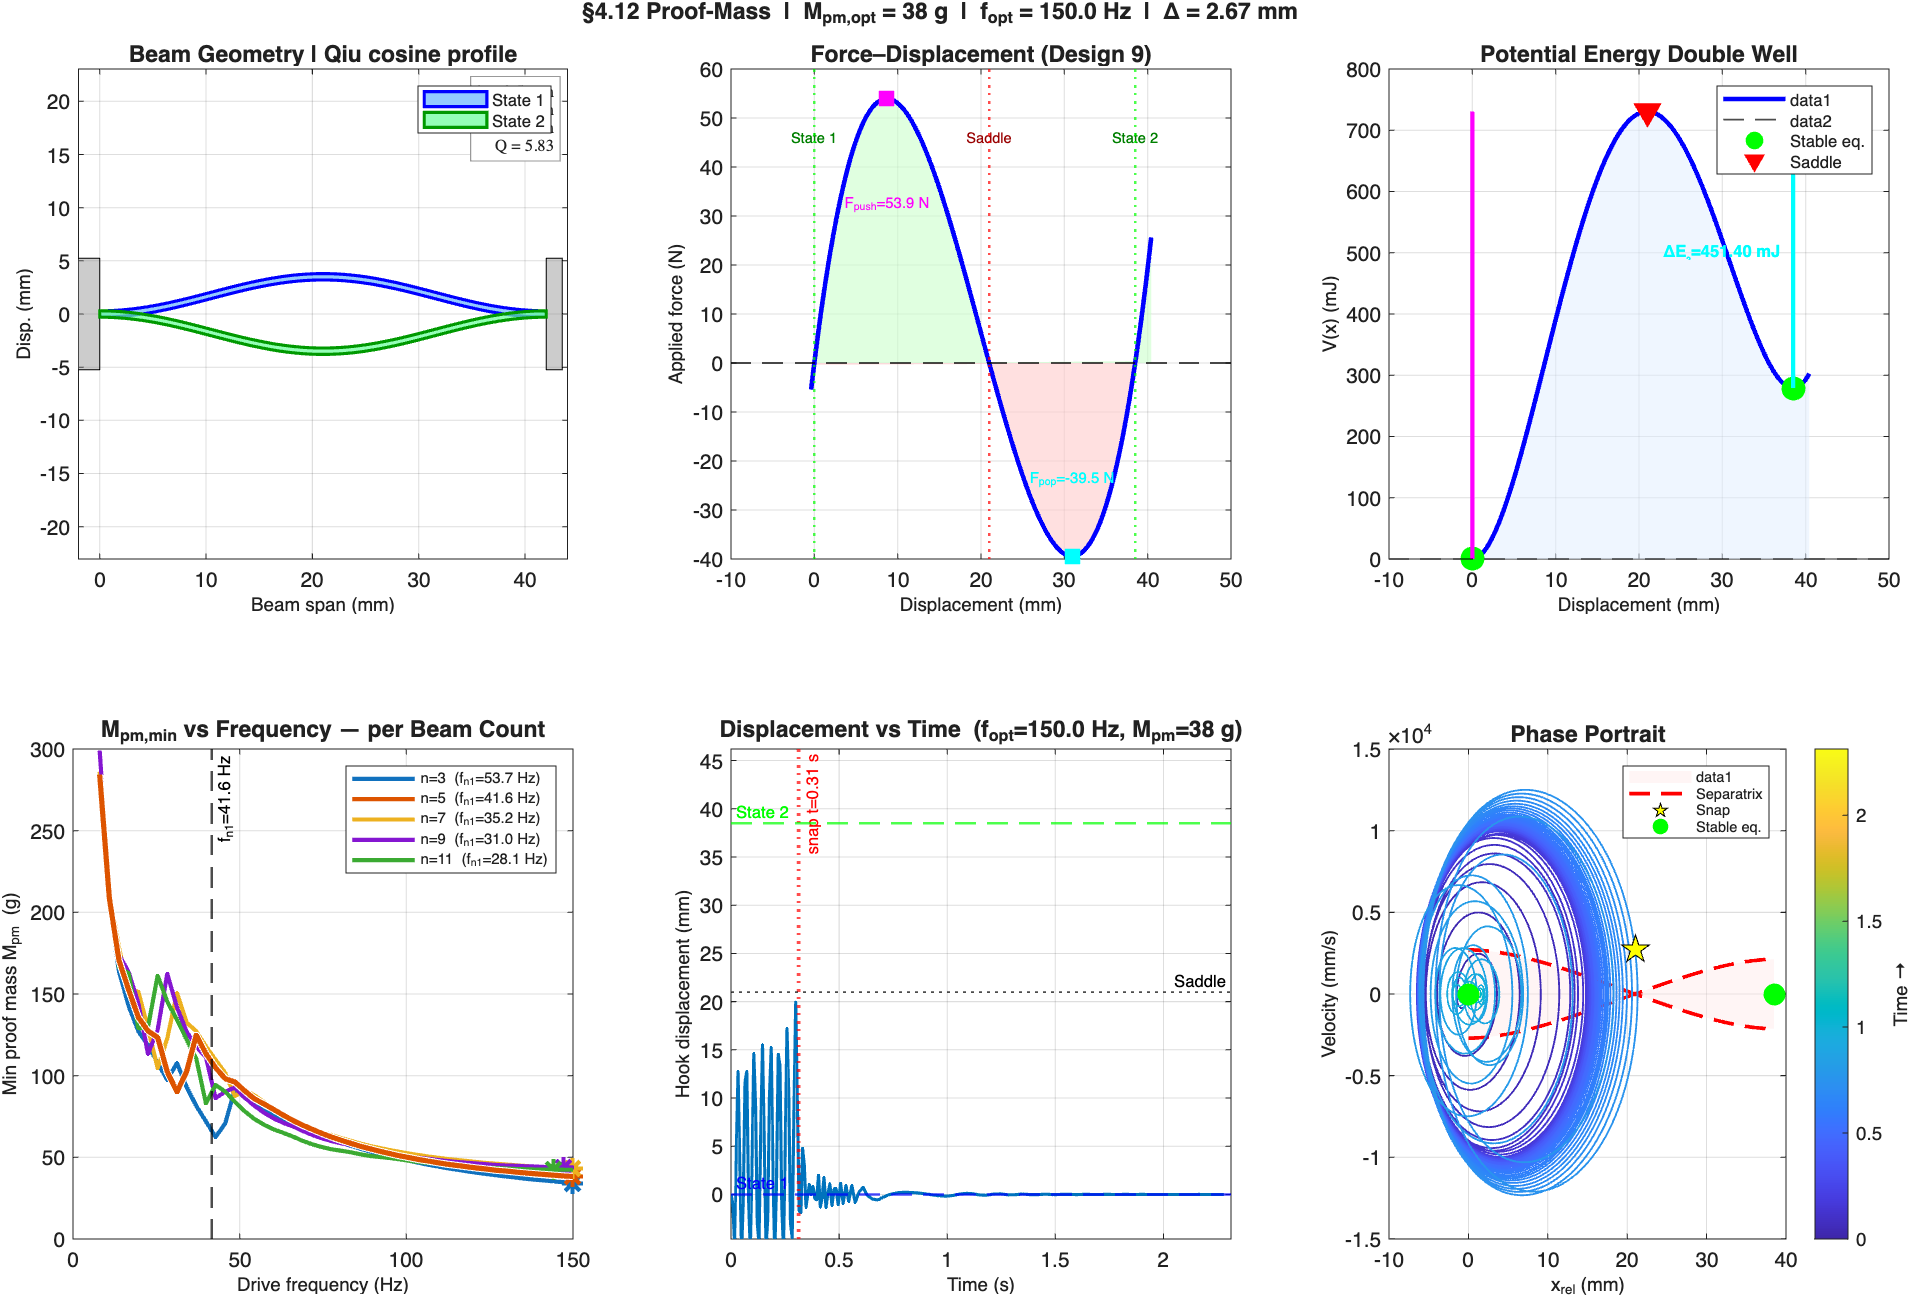
\includegraphics[width=\textwidth]{412_Proof-Mass__Mass_Actuation_Analysis.png}
\caption{Proof-mass actuation analysis: minimum proof mass $M_{pm,\min}$ and
         corresponding snap-through drive frequency as a function of design
         parameters ($N$ parallel beams, hook mass $m_h$).}
\label{fig:pm_analysis}
\end{figure}

\begin{figure}[H]
\centering
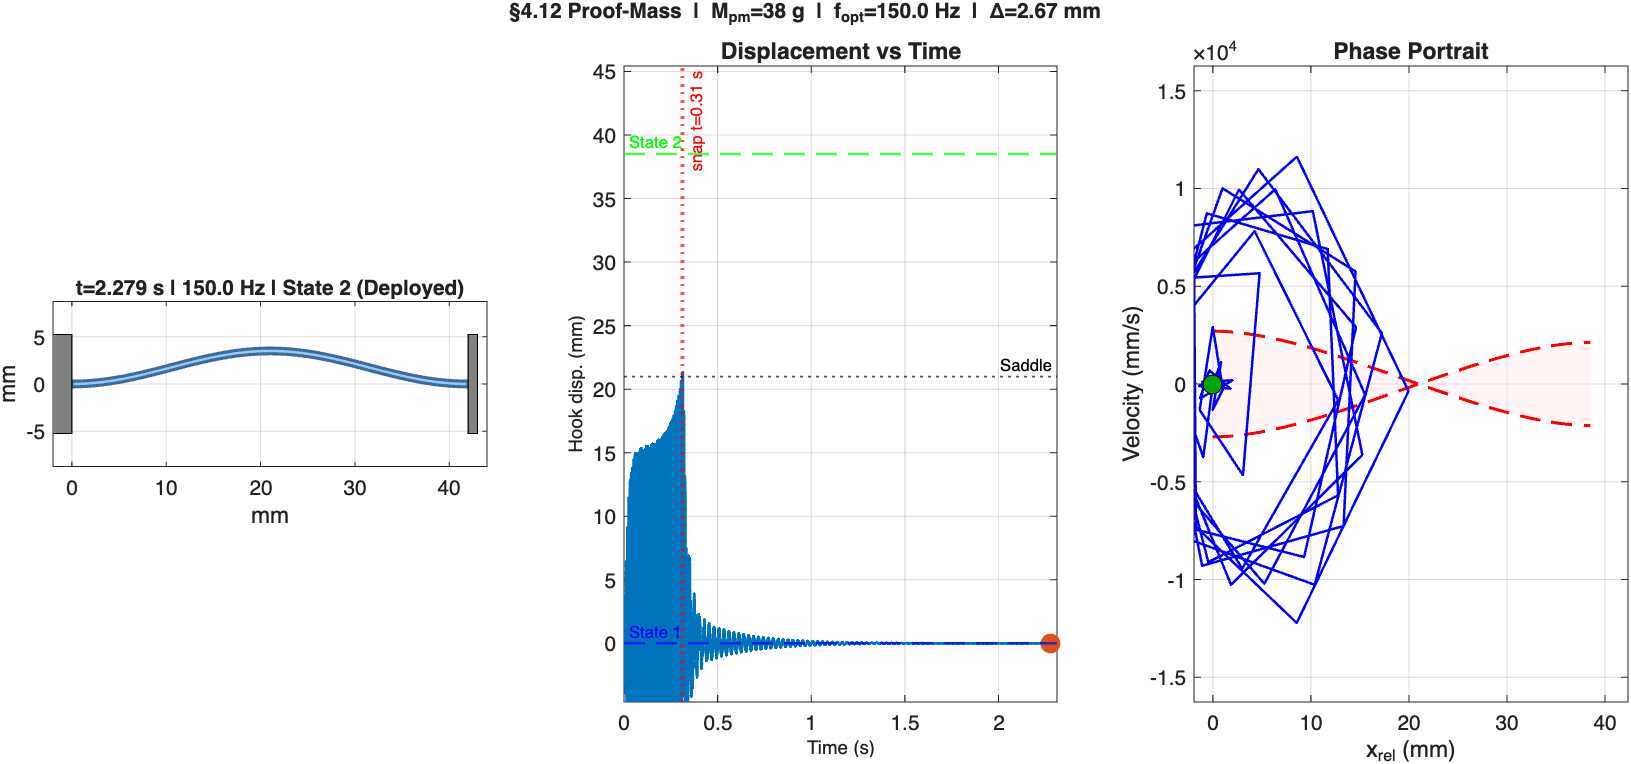
\includegraphics[width=\textwidth]{Bistable_Excitation__Animation__Sec_412_Proof-Mass_Optimal.png}
\caption{Animation snapshot for the Section~\ref{ssec:proof_mass} proof-mass
         actuator at the optimal proof-mass parameter. The proof mass oscillates
         on the motor output shaft, driving the plate and hook into snap-through.}
\label{fig:anim_pm}
\end{figure}

%%─────────────────────────────────────────────────────────────────────────────
\section{Actuator Limit Used in the Simulation}
\label{sec:actuator_limit}
%%─────────────────────────────────────────────────────────────────────────────

The detailed RS05 motor parameters and CAN command notes have been moved to the
separate RS05 notes (\path{rs05_motor_specifications.tex} and
\path{rs05_motor_specifications.typ}). The main derivation only needs the
output-shaft velocity limit used by the proof-mass and prescribed-motion models:
\begin{equation}
  \omega_{\max} = 50.3\;\text{rad/s}.
\end{equation}

For sinusoidal shaft motion at frequency $f$ and angular amplitude $\Theta$,
\begin{equation}
  v_{\mathrm{peak}} = \Theta\,2\pi f \leq \omega_{\max}
  \label{eq:vpeak}
\end{equation}
so the maximum angular amplitude is
\begin{equation}
  \Theta_{\max}(f) = \frac{\omega_{\max}}{2\pi f}
  \label{eq:Thetamax}
\end{equation}
and the corresponding linear stroke through lever arm $r$ is
\begin{equation}
  \delta_{\max}(f) = \frac{\omega_{\max}r}{2\pi f}.
  \label{eq:deltamax}
\end{equation}
For snap-through, the available stroke must reach the saddle $d_s$, so
\begin{equation}
  r_{\min}(f) = \frac{2\pi f d_s}{\omega_{\max}}.
  \label{eq:rmin}
\end{equation}

\section{Optimization}
\label{sec:opt}
%%─────────────────────────────────────────────────────────────────────────────

\subsection{Snap-Through Threshold}
\label{ssec:F0min}

From linear resonance theory, the steady-state hook amplitude at $\omega = \omega_{n,1}$
is:
\begin{equation}
  A_{\mathrm{ss}} = \frac{F_0}{2\zeta_h\,k_{\mathrm{eff},1}}
  \label{eq:Ass}
\end{equation}
Snap-through occurs when $A_{\mathrm{ss}} \geq d_s$, giving:
\begin{equation}
  \boxed{F_{0,\min} = 2\,\zeta_h\,k_{\mathrm{eff},1}\,d_s}
  \label{eq:F0min2}
\end{equation}
This is the \emph{minimum force applied directly at the hook}.  For base
excitation (motor on plate), the motor force required is larger by a factor
that depends on the plate dynamics and drive frequency.

\subsection{Mass Actuation Force}
\label{ssec:mass_actuation}

The central design question for the Rolly deployment mechanism is:
\textit{for a given mass budget added to the robot, what is the maximum
force that mass can deliver to the bistable hook?}

\subsubsection{Proof-Mass Oscillator (Section~\ref{ssec:proof_mass})}

A proof mass $M_{pm}$ oscillating at frequency $\omega$ and amplitude $\Delta$
delivers inertial force $F = M_{pm}\,\Delta\,\omega^2$.  At the velocity limit
(\cref{eq:Thetamax}):
\begin{equation}
  \Delta_{\max}(\omega) = \frac{\omega_{\max}\,r}{\omega}
\end{equation}
The maximum force per unit proof mass is:
\begin{equation}
  \frac{F_{\max}}{M_{pm}} = \Delta_{\max}\,\omega^2
                           = \omega_{\max}\,r\,\omega
  \label{eq:force_per_mass}
\end{equation}
This grows \emph{linearly with drive frequency}.  Higher frequency delivers
more force for the same proof mass — up to the limit imposed by the bistable
dynamics (TMD anti-resonance at $\omega_{n,1}$; see Section~\ref{ssec:case1}).
The coupled relative-mode resonance at $\omega_{\mathrm{rel}}$ is the correct
drive frequency:
\begin{equation}
  \omega_{\mathrm{rel}} = \sqrt{\frac{k_{\mathrm{eff},1}}{M_{\mathrm{red}}}},
  \qquad
  M_{\mathrm{red}} = \frac{m_h\,M_P}{m_h + M_P}
  \label{eq:omrel}
\end{equation}
The minimum proof mass to snap at $\omega_{\mathrm{rel}}$ is found by binary
search over the nonlinear ODE.

\begin{figure}[H]
\centering
\begin{subfigure}[b]{0.49\textwidth}
  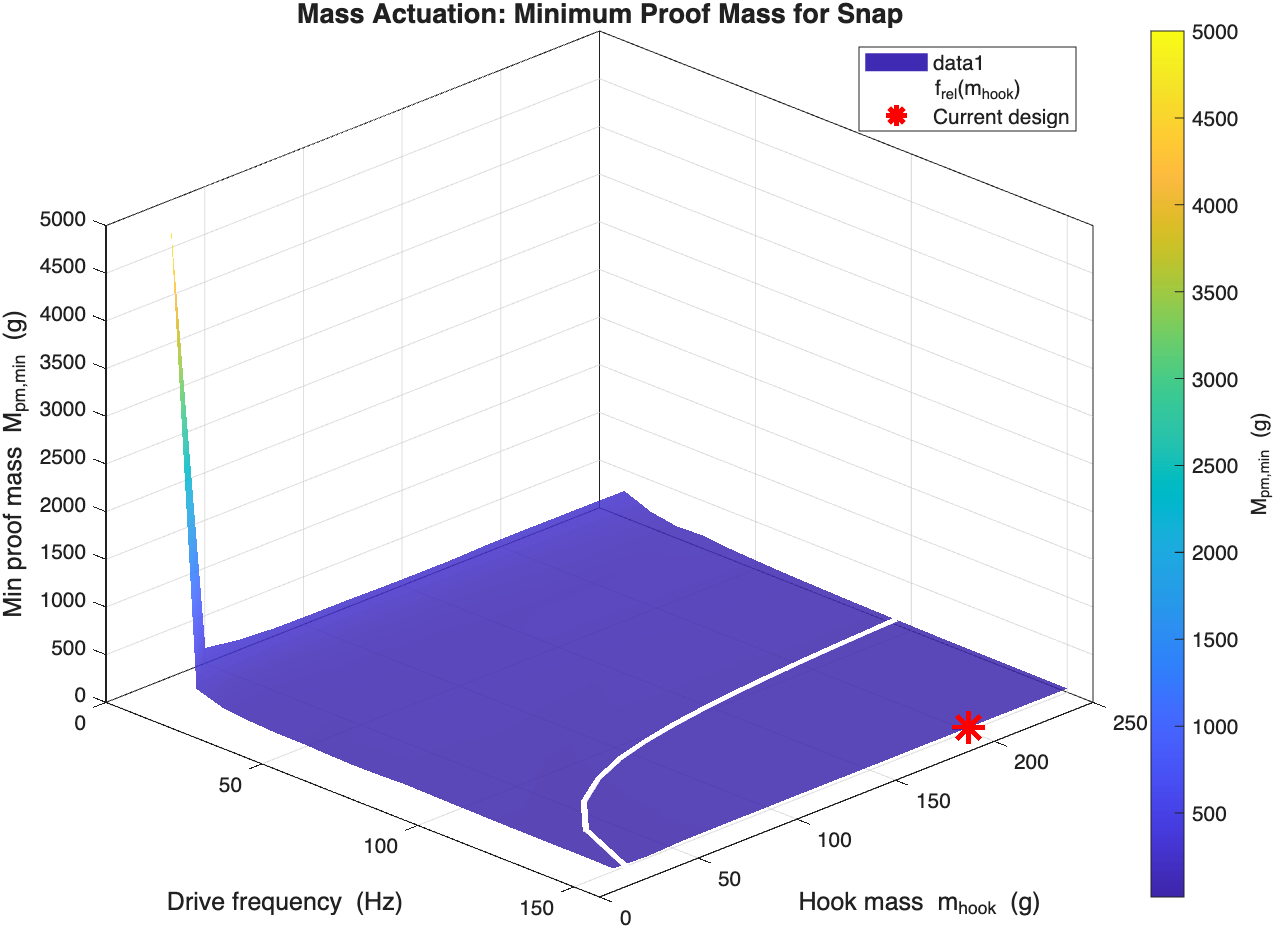
\includegraphics[width=\textwidth]{3-D_M_pmminf_drive_m_hook.png}
  \caption{$M_{pm,\min}$ vs.\ drive frequency and hook mass $m_h$.}
  \label{fig:3d_pm_mhook}
\end{subfigure}\hfill
\begin{subfigure}[b]{0.49\textwidth}
  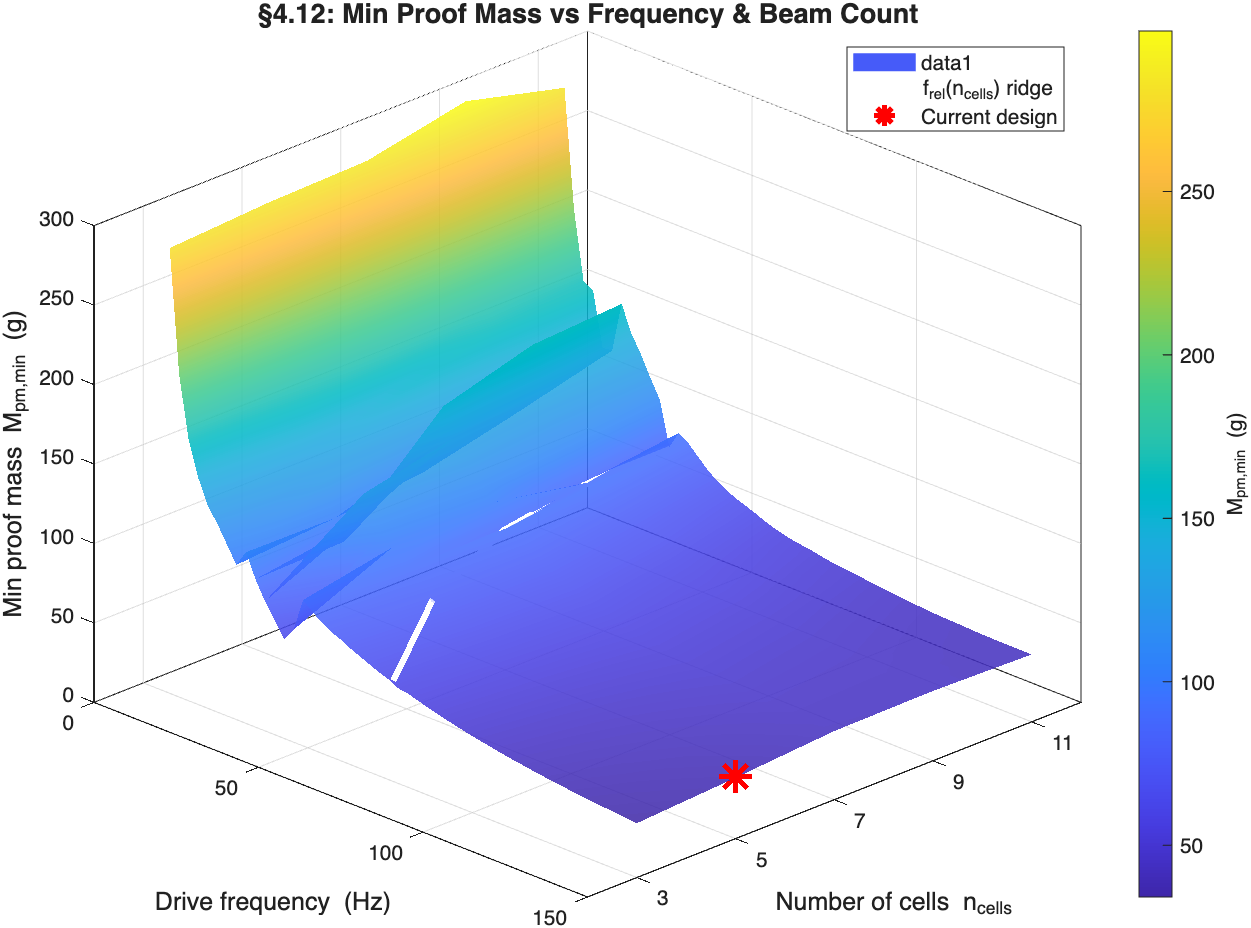
\includegraphics[width=\textwidth]{3-D_M_pmminf_drive_n_cells.png}
  \caption{$M_{pm,\min}$ vs.\ drive frequency and number of parallel beams $N$.}
  \label{fig:3d_pm_ncells}
\end{subfigure}
\caption{3-D design surfaces for the minimum required proof mass $M_{pm,\min}$
         to achieve snap-through, swept over the drive frequency and two key
         design variables.  Each surface is obtained by binary search over the
         nonlinear ODE at every grid point.}
\label{fig:3d_pm}
\end{figure}

\subsubsection{Config~2: Prescribed Base Motion (no added mass)}

The motor prescribes the plate displacement $x_P(t) = A\sin(\omega_{n,1}t)$.
The minimum plate amplitude for resonant snap is:
\begin{equation}
  A_{\min} = 2\,\zeta_h\,d_s
  \label{eq:Amin_c2}
\end{equation}
The required motor torque at resonance ($\omega = \omega_{n,1}$):
\begin{equation}
  \tau = m_h\,A_{\min}\,\omega_{n,1}^2\,r
       = 2\,\zeta_h\,k_{\mathrm{eff},1}\,d_s\,r
  \label{eq:tau_c2}
\end{equation}
This is \emph{independent of hook mass} $m_h$.  No additional hardware
mass is required --- the motor already present for locomotion is used.

\begin{figure}[H]
\centering
\begin{subfigure}[b]{0.49\textwidth}
  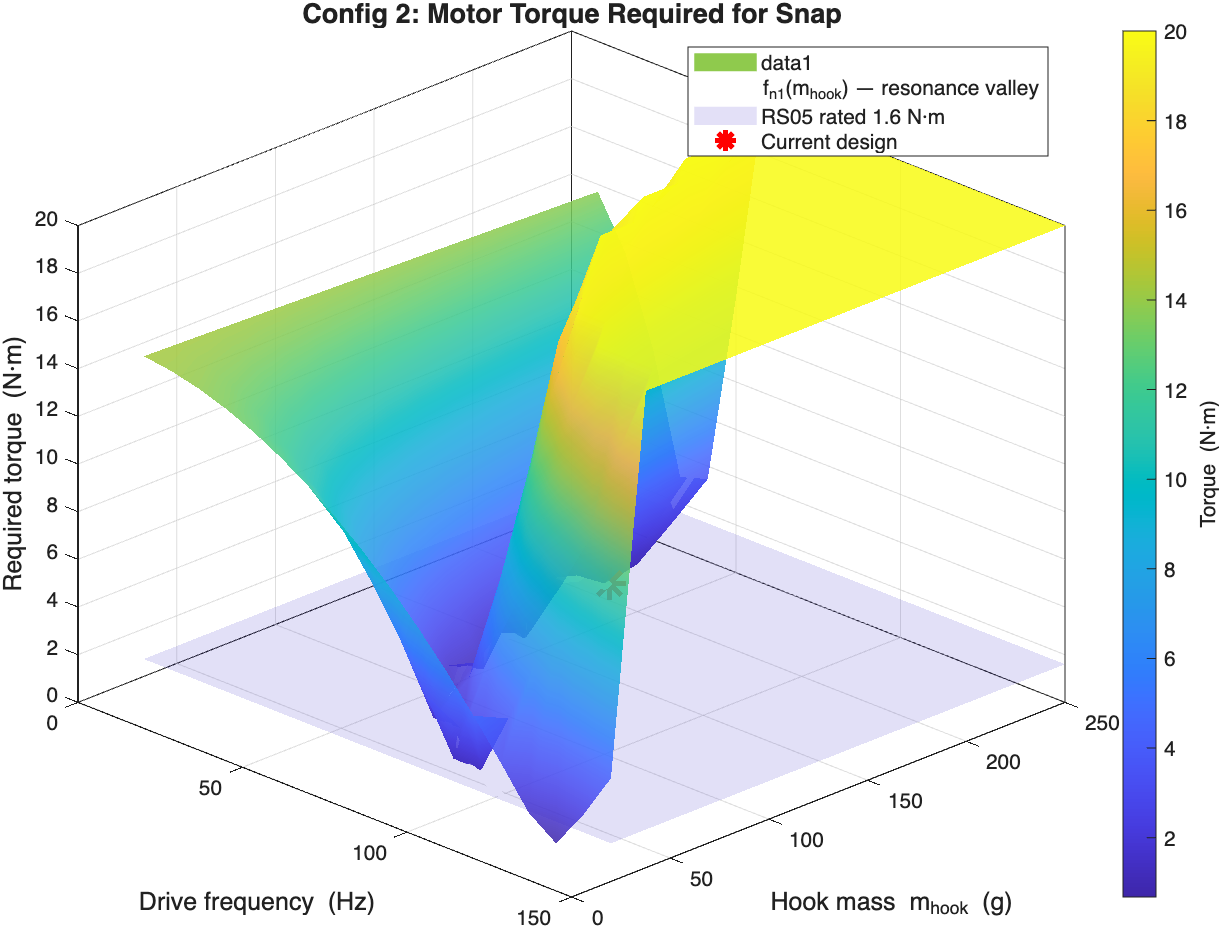
\includegraphics[width=\textwidth]{3-D_Torquef_drive_m_hook__Config_2.png}
  \caption{Required torque vs.\ drive frequency and hook mass $m_h$.}
  \label{fig:3d_tau_mhook}
\end{subfigure}\hfill
\begin{subfigure}[b]{0.49\textwidth}
  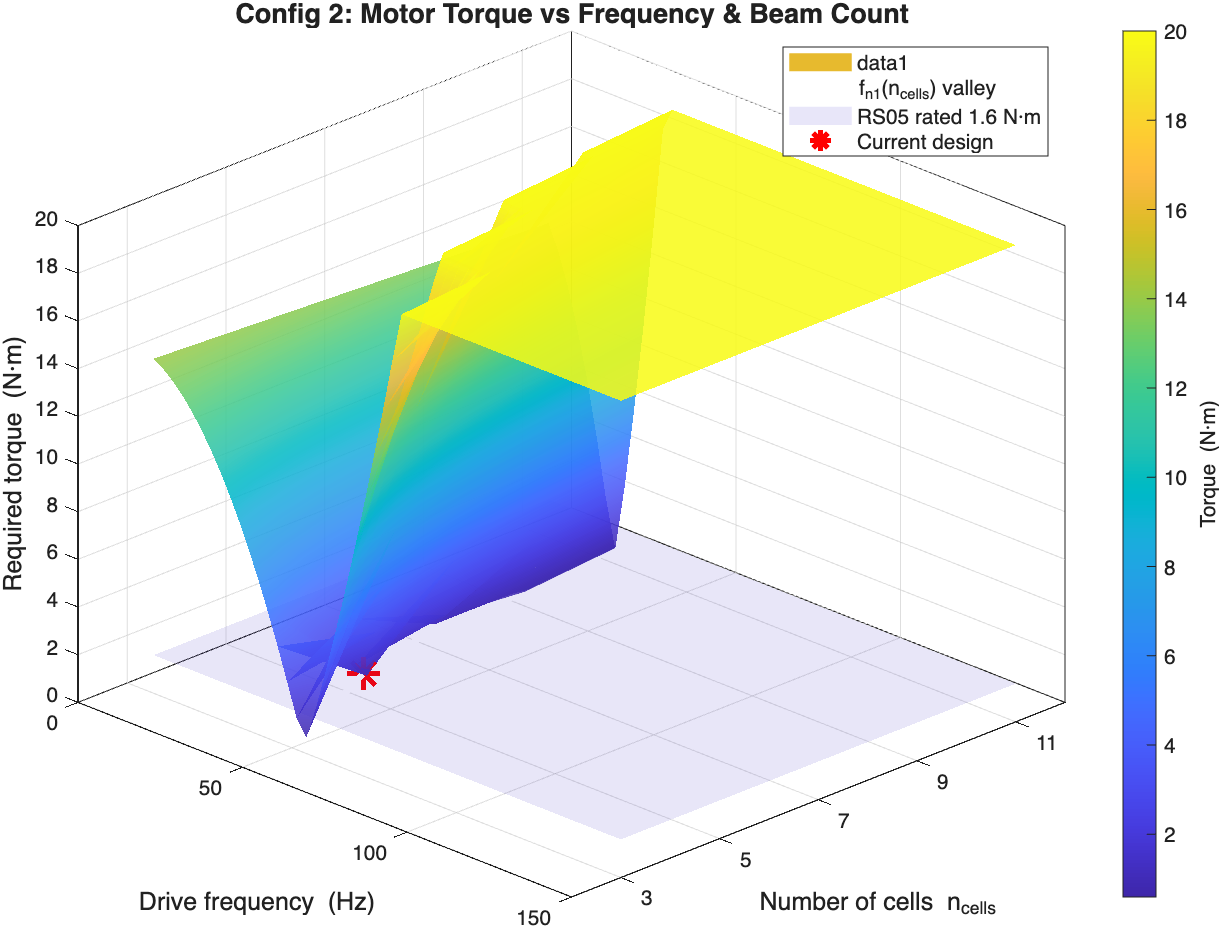
\includegraphics[width=\textwidth]{3-D_Torquef_drive_n_cells__Config_2.png}
  \caption{Required torque vs.\ drive frequency and number of parallel beams $N$.}
  \label{fig:3d_tau_ncells}
\end{subfigure}
\caption{3-D design surfaces for the required motor torque under
         Configuration~2 (prescribed base motion) for snap-through, swept over
         the drive frequency and two key design variables.}
\label{fig:3d_tau}
\end{figure}

\subsection{Parallel Beam-Count Scaling (\texorpdfstring{$N$}{N} beams)}
\label{ssec:ncells}

For the current model, $N$ is the number of parallel bistable beams. The beams
share the same hook displacement, so adding beams increases force and stiffness,
not stroke:
\begin{align}
  d_f &= d_{f,1} \quad\text{(stroke unchanged)}\\
  d_s &= d_{s,1} \quad\text{(saddle unchanged)}\\
  k_{\mathrm{eff},1} &\propto N \quad\text{(stiffness rises)}\\
  f_{n,1} &\propto \sqrt{N} \quad\text{(natural frequency rises)}\\
  F_{0,\min} &\propto N \quad\text{(force threshold rises)}
\end{align}
The old series assumption made the saddle displacement look too large. In the
parallel model, $N=5$ raises the stored energy and stiffness while keeping the
hook travel at the single-beam value.

The post-snap potential energy available to accelerate the hook to State~2 is
\begin{equation}
  \Delta E_2 = V(d_s) - V(d_f).
\end{equation}
It grows with $N$ because the force-displacement curve scales upward, not
because the stroke grows.

\subsection{Impact Force at State 2}
\label{ssec:impact}

When the hook arrives at $x_{\mathrm{rel}} = d_f$ it has kinetic energy
accumulated from two sources:
\begin{enumerate}[nosep]
  \item \textbf{Kinetic energy at saddle crossing} $KE_{\mathrm{saddle}}$
    (from resonant build-up).
  \item \textbf{Potential energy released} by the bistable spring from saddle
    to State~2: $\Delta E_2$.
\end{enumerate}
The hook velocity at impact (ignoring damping over the short snap transit):
\begin{equation}
  v_{\mathrm{impact}} = \sqrt{v_{\mathrm{saddle}}^2 + \frac{2\,\Delta E_2}{m_h}}
  \label{eq:vimpact}
\end{equation}
At the minimum snap threshold $v_{\mathrm{saddle}} \approx 0$, so
$v_{\mathrm{impact}} \approx \sqrt{2\,\Delta E_2 / m_h}$.

The peak force on the target object (Hertz contact model):
\begin{equation}
  F_{\mathrm{peak}} = v_{\mathrm{impact}}\,\sqrt{k_{\mathrm{contact}}\,m_h}
  \label{eq:Fpeak}
\end{equation}
where $k_{\mathrm{contact}}$ is the contact stiffness.  The impact force
scales as $\sqrt{k_{\mathrm{contact}}}$: steel-on-steel
($k \sim 10^{10}$\,N/m) gives $\sim 3000\times$ more peak force than
rubber-on-rubber ($k \sim 10^{4}$\,N/m) for the same impact velocity.

The impact momentum (relevant for deforming targets):
\begin{equation}
  p = m_h\,v_{\mathrm{impact}} = \sqrt{2\,m_h\,\Delta E_2}
  \label{eq:pimpact}
\end{equation}
grows as $\sqrt{m_h}$ — heavier hooks deliver more momentum.

%%─────────────────────────────────────────────────────────────────────────────
\section{Nomenclature}
\label{sec:nomenclature}
%%─────────────────────────────────────────────────────────────────────────────

\begingroup
\renewcommand{\arraystretch}{1.25}
\small
\begin{longtable}{p{2.1cm} p{1.5cm} p{6.7cm} p{3.1cm}}
\caption{Symbol definitions used in this document and the MATLAB simulations.}
\label{tab:nomenclature}\\
\toprule
\textbf{Symbol} & \textbf{Unit} & \textbf{Description} & \textbf{Typical value} \\
\midrule
\endfirsthead
\toprule
\textbf{Symbol} & \textbf{Unit} & \textbf{Description} & \textbf{Typical value} \\
\midrule
\endhead
\midrule
\multicolumn{4}{r}{\textit{continued on next page}}\\
\endfoot
\bottomrule
\endlastfoot
\multicolumn{4}{l}{\textit{Simulation 2 — Curved-beam bistable}} \\
$E$        & Pa      & Elastic modulus (ABS)         & 2300$\times10^6$ \\
$t$        & m       & Beam thickness                & 0.6$\times10^{-3}$ \\
$h$        & m       & Beam apex height              & 3.5$\times10^{-3}$ \\
$l$        & m       & Beam span                     & 42$\times10^{-3}$ \\
$Q$        & ---     & Apex-height-to-thickness ratio & $h/t$ (target $\gtrsim2.35$) \\
$N$        & ---     & Number of parallel beams      & 5 \\
$d_f$      & m       & Mechanism stroke              & 7.70$\times10^{-3}$ \\
$d_s$      & m       & Saddle position               & $0.545\,d_f$ \\
$A$        & N/m$^3$ & Cubic polynomial coefficient  & from \cref{eq:Acoeff} \\
$F_{\mathrm{push}}$ & N & Peak push force (beam pack) & $N\times52.4$ (current model) \\
$F_{\mathrm{pop}}$  & N & Valley force               & from cubic fit \\
$k_{\mathrm{eff,1}}$ & N/m & Stiffness at State~1   & $A\,d_s\,d_f$ \\
$k_{\mathrm{eff,2}}$ & N/m & Stiffness at State~2   & $A\,d_f(d_f-d_s)$ \\
$f_{n,1}$  & Hz      & Natural freq.\ at State~1     & $\omega_{n,1}/(2\pi)$ \\
$f_{n,2}$  & Hz      & Natural freq.\ at State~2     & $\omega_{n,2}/(2\pi)$ \\
$m_1$      & kg      & Main mass (TMD model)         & 0.150 \\
$m_2$      & kg      & TMD mass                      & 0.01875 \\
$k_{\mathrm{main}}$ & N/m & Main spring stiffness   & 7253 (35 Hz) \\
$E_r$      & Pa      & Ruler elastic modulus         & 210$\times10^9$ \\
\midrule
\multicolumn{4}{l}{\textit{Section 3 — Base excitation model}} \\
$x_P$      & m       & Absolute plate displacement   & (simulated) \\
$x_{\mathrm{rel}}$ & m & Hook displacement relative to plate & (simulated) \\
$M_P$      & kg      & Plate + bistable assembly mass (motor excluded) & 0.200 \\
$f_P$      & Hz      & Plate support natural frequency & set to $f_{n,1}$ \\
$\zeta_P$  & ---     & Plate structural damping ratio & 0.02 \\
$k_s$      & N/m     & Plate support stiffness       & $M_P(2\pi f_P)^2$ \\
$c_s$      & N$\cdot$s/m & Plate support damping     & $2\zeta_P M_P(2\pi f_P)$ \\
$F_0$      & N       & Motor force amplitude at plate & $\tau_{\mathrm{out}}/r_{\mathrm{arm}}$ \\
$\tau_{\mathrm{out}}$ & N$\cdot$m & Measured RS05 output torque (from T-N curve) & $\leq 5.5$ \\
$r_{\mathrm{arm}}$ & m & Coupling moment arm          & 0.010 \\
$n_g$      & ---     & RS05 planetary gear ratio     & 7.75 \\
$J_{\mathrm{eff}}$ & kg$\cdot$m$^2$ & Reflected rotor inertia at output & $J_{\mathrm{rotor}}\,n_g^2$ \\
$f_{\mathrm{cut}}$ & Hz & Gearbox low-pass cut-off frequency & $\frac{1}{2\pi}\sqrt{k_{\mathrm{gear}}/J_{\mathrm{eff}}}$ \\
$f_{\mathrm{mesh}}$ & Hz & Gear-mesh frequency          & $n_g f_{\mathrm{rotor}} N_{\mathrm{teeth}}$ \\
$n$        & ---     & Detuning ratio $f_P/f_{n,1}$  & 1 (tuned) \\
$Q_P$      & ---     & Plate quality factor $1/(2\zeta_P)$ & 25 \\
$Q_h$      & ---     & Hook quality factor $1/(2\zeta_h)$ & 10 \\
\midrule
\multicolumn{4}{l}{\textit{Section 5 — Optimization and mass actuation}} \\
$N$        & ---     & Number of parallel bistable beams & 5 \\
$f_{\mathrm{rel}}$ & Hz & Coupled relative-mode resonance $= \sqrt{k_{\mathrm{eff},1}/M_{\mathrm{red}}}/(2\pi)$ & 22 \\
$M_{\mathrm{red}}$ & kg & Reduced mass $= m_h M_P/(m_h+M_P)$ & 0.133 \\
$M_{pm}$   & kg      & Proof mass (oscillating on motor shaft) & optimised \\
$\Delta$   & m       & Proof-mass oscillation amplitude & velocity-limited \\
$\omega_{\max}$ & rad/s & RS05 max shaft angular velocity (480 RPM) & 50.3 \\
$M_{pm,\min}$ & kg   & Minimum proof mass to snap at given $(f,N)$ & from sweep \\
$A_{\min}$ & m       & Minimum plate amplitude for Config~2 snap & $2\zeta_h d_s$ \\
$\tau_{C2}$ & N$\cdot$m & Config~2 motor torque $= 2\zeta_h k_{\mathrm{eff}} d_s r$ & 2.87 \\
$\Delta E_2$ & J     & Post-snap potential energy released (saddle to State~2) & grows with $N$ \\
$v_{\mathrm{impact}}$ & m/s & Hook velocity at State~2 impact & $\sqrt{2\Delta E_2/m_h}$ \\
$k_{\mathrm{contact}}$ & N/m & Target contact stiffness (Hertz) & $10^4$--$10^{10}$ \\
$F_{\mathrm{peak}}$ & N & Peak impact force $= v_{\mathrm{impact}}\sqrt{k_c m_h}$ & --- \\
\end{longtable}
\endgroup

%%─────────────────────────────────────────────────────────────────────────────
\section*{References}
%%─────────────────────────────────────────────────────────────────────────────

\begin{thebibliography}{99}

\bibitem{nayfeh1979}
A.~H.~Nayfeh and D.~T.~Mook,
\textit{Nonlinear Oscillations},
Wiley-Interscience, New York, 1979.

\bibitem{denhartog1956}
J.~P.~Den Hartog,
\textit{Mechanical Vibrations}, 4th~ed.,
McGraw-Hill, New York, 1956.

\bibitem{qiu2003}
J.~Qiu, A.~H.~Slocum, J.~H.~Lang, R.~Struempler, M.~P.~Brenner, and J.~Li,
\textit{Bistable Actuation Techniques, Mechanisms, and Applications},
U.S.\ Patent Application Publication US~2003/0029705~A1,
Feb.\ 2003.

\bibitem{qiu2004}
J.~Qiu, J.~H.~Lang, and A.~H.~Slocum,
``A Curved-Beam Bistable Mechanism,''
\textit{Journal of Microelectromechanical Systems}, vol.~13, no.~2,
pp.~137--146, 2004.
\url{https://doi.org/10.1109/JMEMS.2004.825308}

\bibitem{zolfagharian2025}
A.~Zolfagharian, F.~Demoly, M.~Lakhi, B.~Rolfe, and M.~Bodaghi,
``Bistable Mechanisms 3D Printing for Mechanically Programmable Vibration Control,''
\textit{Advanced Engineering Materials}, vol.~28, no.~9, p.~2402233, 2026.
\url{https://doi.org/10.1002/adem.202402233}

\bibitem{liu2023}
Y.~Liu, J.~Zhang, D.~Pan, Z.~Wu, and Q.~Wang,
``Resonant Actuation Based on Dynamic Characteristics of Bistable Laminates,''
\textit{Machines}, vol.~11, no.~3, p.~318, 2023.
\url{https://doi.org/10.3390/machines11030318}

\bibitem{robstride2026}
RobStride,
\textit{RS05 User Manual}, Rev.~260428, 2026.

\end{thebibliography}

\end{document}
